%% Focal Point Review for Applied Spectroscopy (Sage). Plain article class: the journal
%% requires no template, only clear headings. References: numbered superscripts; Applied Spectroscopy bibliography style.
\documentclass[12pt,a4paper]{article}
\usepackage[T1]{fontenc}
\usepackage[utf8]{inputenc}
\usepackage[margin=2.5cm]{geometry}
\usepackage{setspace}\doublespacing
\usepackage{amsmath,amssymb}
\usepackage{newtxtext,newtxmath}
\usepackage{graphicx}
\usepackage{caption}
\captionsetup{font={normalsize,stretch=2},labelfont=bf,labelsep=period,justification=raggedright,singlelinecheck=false}
\renewenvironment{abstract}{\par\noindent\textbf{Abstract}\par\noindent\normalsize}{\par\medskip}
% Shared caption text: displayed below each figure and in the final list required by Applied Spectroscopy.
\newcommand{\FigureCaptionOne}{Composition of the 138 documents cited in the review: 111 analyzed device studies, grouped into six hardware families, and 27 supporting documents.}
\newcommand{\FigureCaptionTwo}{Typical transmission layouts of the six hardware families: (a) LED photometers and colorimeters, (b) smartphone grating spectrometers, (c) camera/SBC grating spectrometers, (d) mini-spectrometer modules, (e) multispectral sensor chips, and (f) a scanning-grating design. In each row, the shaded block marks the element that selects the wavelengths (in (a), the LED itself); the different tints only help to tell the families apart. White blocks are elements shared by several families. Reflectance geometries are not shown. S, sample; MCU, microcontroller; SBC, single-board computer; PC, personal computer.}
\newcommand{\FigureCaptionThree}{The three systems compared in this work: (a) system A, an AS7265x multispectral sensor controlled by an ESP32; (b) system B, a Raspberry Pi camera coupled to a pocket spectroscope; (c) system C, the Little Garden webcam spectrometer.}
\newcommand{\FigureCaptionFour}{Reference absorbance spectra of nine of the eleven dye solutions, measured with the Genesys~30 spectrophotometer (orange and pink are not shown). Lemon and rose exceed 2.5, the upper limit of the specified photometric accuracy.}
\newcommand{\FigureCaptionFive}{Absorbance spectra of the blue, green, and red validation dyes: (a) reference spectrophotometer (Genesys~30); (b)--(d) systems A, B, and C before (dashed) and after (solid) absorbance calibration. Symbols in (b) mark the 11 channels of A, and connecting lines are visual guides. Error bars for A and shaded bands for B and C show $\pm$1~SD of 100 readings.}
\newcommand{\FigureCaptionSix}{Reference absorbance plotted against calibrated absorbance for systems (a) A, (b) B, and (c) C, for the three validation dyes over 400--700~nm. Each point is one wavelength of one dye, colored by wavelength; the gray line is the identity.}
\newcommand{\FigureCaptionSeven}{Reported cost totals for 56 analyzed device studies by hardware family. Marker shape shows what the cost covers, small downward-pointing triangles mark upper price bounds and stars show systems A, B, and C. Amounts were converted at 1~EUR = 1.10~USD, 1~GBP = 1.27~USD, and 1~SGD = 0.74~USD, without adjusting for inflation.}

\newcommand{\PrintFigureCaptions}{%
\clearpage
\section*{Figure captions}
\noindent\textbf{Figure 1.} \FigureCaptionOne\par\medskip
\noindent\textbf{Figure 2.} \FigureCaptionTwo\par\medskip
\noindent\textbf{Figure 3.} \FigureCaptionThree\par\medskip
\noindent\textbf{Figure 4.} \FigureCaptionFour\par\medskip
\noindent\textbf{Figure 5.} \FigureCaptionFive\par\medskip
\noindent\textbf{Figure 6.} \FigureCaptionSix\par\medskip
\noindent\textbf{Figure 7.} \FigureCaptionSeven\par\medskip
}

\graphicspath{{figures/}}
\usepackage{booktabs}
\usepackage{tabularx}
\usepackage{xltabular}
\usepackage{needspace}
\usepackage{eurosym}
\usepackage{textcomp}
\usepackage{float}
\usepackage{placeins}
% Allow text beside the page allocation for large figures; avoid half-empty float pages.
\renewcommand{\topfraction}{0.9}
\renewcommand{\bottomfraction}{0.8}
\renewcommand{\textfraction}{0.07}
\renewcommand{\floatpagefraction}{0.85}
\usepackage{xurl}
\usepackage[super,comma,sort&compress]{natbib}
\renewcommand{\bibnumfmt}[1]{#1.}
\usepackage{authblk}
\usepackage{etoolbox}
\AtBeginEnvironment{table}{\doublespacing}
\usepackage{lineno}\linenumbers
\setlength{\emergencystretch}{3em}
\clubpenalty=10000
\widowpenalty=10000
\displaywidowpenalty=10000
\setcounter{secnumdepth}{-1}
\renewcommand{\thetable}{\Roman{table}}

\usepackage{xcolor}
\usepackage[hidelinks]{hyperref}


\title{Low-Cost Spectrophotometers: Architectures, Calibration, Validation, and Reproducibility}

\author[1,2,3]{Alex M. Rivera-Rivera}
\author[3,2]{Daniela Martinez-Ortiz}
\author[4]{Fran\c{c}ois Quitin}
\author[5,6]{Denis Terwagne}
\author[7]{Stamatios C. Nicolis}
\author[3]{Ernesto Altshuler}
\author[7]{Alexandre Campo}
\affil[1]{Innovation Laboratory, Technological University of Havana Jos\'e Antonio Echeverr\'ia (CUJAE), 19390 Havana, Cuba}
\affil[2]{Facult\'e des Sciences, Universit\'e Libre de Bruxelles (ULB), 1050 Brussels, Belgium}
\affil[3]{Center for Complex Systems, Physics Faculty, University of Havana, 10400 Havana, Cuba}
\affil[4]{Brussels School of Engineering, Universit\'e libre de Bruxelles, Avenue Franklin Roosevelt 50, 1000 Brussels, Belgium}
\affil[5]{Frugal Lab, D\'epartement de physique, Facult\'e des Sciences, Universit\'e libre de Bruxelles (ULB), 1050 Brussels, Belgium}
\affil[6]{Fab Lab ULB, Universit\'e libre de Bruxelles (ULB), 1050 Brussels, Belgium}
\affil[7]{Unit of Biological and Artificial Self-organizing Systems, Department of Physical Chemistry and Theoretical Biology, Center for Nonlinear Phenomena and Complex Systems, Universit\'e libre de Bruxelles, Bd du Triomphe, 1050 Brussels, Belgium}
\date{}

\begin{document}
\maketitle

\noindent\textbf{Corresponding author:} Alex M. Rivera-Rivera (\texttt{alex.rivera.rivera@ulb.be})

\begin{abstract}
We examined 111 studies, published from 2012 onward, that describe low-cost ultraviolet, visible, or near-infrared spectrophotometers, and traced how optical design, calibration, validation, cost, and openness vary across six hardware families. Just under half of these studies tested their instruments on samples that had not been used for calibration, a similar share reported how repeatable the readings were, and only about a quarter shared design files or code. Since the studies measured different targets, evaluated them in different ways, and counted costs differently, they cannot be used to rank the hardware families against one another. To complement the literature, we compared three instruments with a laboratory spectrophotometer under a single protocol: an AS7265x multispectral sensor (system A), a Raspberry Pi camera behind a pocket grating spectroscope (system B), and a commercial webcam grating spectrometer (system C). On three food-dye solutions kept out of calibration fitting and model selection, the root-mean-square absorbance differences over 400--700~nm were 0.281, 0.077, and 0.094, respectively. These figures describe the particular units and acquisition procedures we tested. We end with an application-dependent reporting checklist meant to help readers decide whether a low-cost instrument suits a given measurement, and to help others rebuild it.
\end{abstract}

\noindent\textbf{Keywords:} Low-cost spectrophotometry; Open-source instrumentation; Ultraviolet--visible spectroscopy; UV--Vis spectroscopy; Multispectral sensors; Absorbance calibration; Method validation; Reproducibility

\section{Introduction}\label{sec:intro}

Cheap optoelectronic parts and openly shared construction files have put spectrophotometry within reach of classrooms, small laboratories, and field teams.\citep{pereira2019low,laganovska2020portable,feng2021open} Building an instrument is no longer the hard part. The harder question is whether a particular instrument is good enough for the measurement it is supposed to make, and the published figures do not always settle it. Camera-based devices, for instance, can yield linear concentration calibrations even when their absorbance readings differ substantially from those of a laboratory spectrophotometer,\citep{grasse2015teaching,bruininks2022inexpensive} which is why a high calibration $R^2$ tells us little about how accurately new samples will be measured.\citep{prairie2020accurate,cirrone2026analytical}

Earlier reviews have dealt with parts of this field: smartphone spectrometers,\citep{mcgonigle2018smartphone} miniaturized near-infrared (NIR) instruments,\citep{bec2022miniaturized} chip-scale spectrometers,\citep{yang2021miniaturization} instruments for chemistry teaching,\citep{shidiq2020simple} and the validation of freshwater sensors.\citep{cirrone2026analytical} In this review we bring these strands together and ask how the way an instrument is built relates to what it has been shown to do, and to how easily someone else could reproduce it. We sort the instruments into six hardware families: light-emitting-diode (LED) photometers and colorimeters, smartphone grating spectrometers, camera grating spectrometers, integrated spectrometer modules, multispectral sensor chips, and a small group of other designs. To see how some of these issues play out in practice, we also measured three inexpensive instruments, which we refer to as systems A, B, and C, against a laboratory spectrophotometer using a common absorbance protocol. Both the literature and our own measurements then feed into a reporting checklist whose items depend on the intended application.

\subsection{Literature search and selection}\label{sec:method}

The review cites 138 documents (Figure~\ref{fig:sources}). Of these, 111 are device studies, and all counts and comparisons in the review are based on them; the remaining 27 are supporting documents. Among the supporting documents, 15 came from the literature search, seven are additional contextual or methodological references, and five are technical documents such as instrument specifications, a sensor datasheet, and software documentation.

We searched the literature in October 2026 by two routes. The first was a set of 18 OpenAlex queries restricted to publications from 1 January 2015 onward; keeping the first 50 results of each query yielded 789 unique records. The second route followed the reference lists of selected reviews and the works citing McGonigle et al., Geng et al., Cirrone et al., and Coppola et al.,\citep{mcgonigle2018smartphone,geng2017recent,cirrone2026analytical,coppola2024i} supplemented by nine targeted queries on multispectral chips, and yielded 1325 unique records. Because citation searching also reached older work, the corpus goes back to 2012.

We included English-language journal articles and full conference papers that describe low-cost ultraviolet (UV), visible, or NIR instruments for absorbance, transmittance, or reflectance measurements, including instruments built around commercial spectral modules. No price ceiling was imposed. An instrument counted as low cost when its authors described it that way and its construction was consistent with that description. As a result, reported totals range from about USD~1 to 1100 and cover quite different sets of equipment. Studies of individual components and radiometric characterizations served as supporting evidence on spectral response and stability.

We excluded fluorescence-only, Raman, laser-induced breakdown, and imaging-only instruments, as well as on-chip computational spectrometers, preprints, conference abstracts, and assays carried out only with commercial instruments. Cameras were eligible if they recorded spectra or if their images were synchronized with a separate point spectrum. These criteria defined the device corpus; the contextual engineering references played a supporting role only.

For every study we recorded the design, components, spectral capability, calibration, samples, reference comparisons, performance, cost, and availability of files. A characteristic was counted only if the study documented it explicitly. One author extracted the data and coded each study, and a second author checked the coding; disagreements were resolved by discussion. The queries, screening records, definitions, and source evidence are available from the authors on reasonable request.

\begin{figure}[!htbp]
\centering
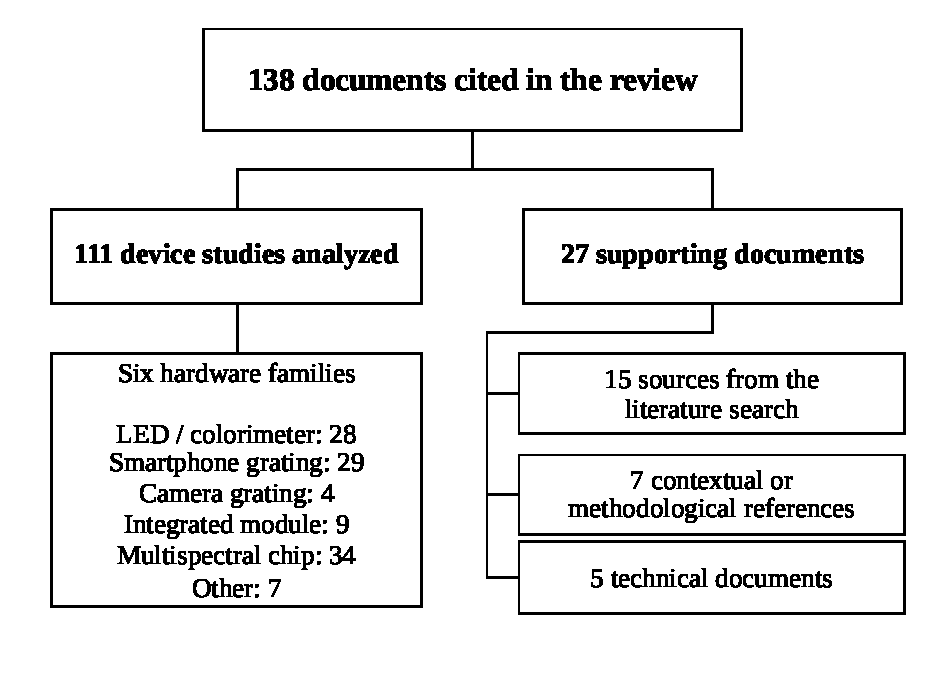
\includegraphics[width=\linewidth]{prisma.pdf}
\caption{\FigureCaptionOne}\label{fig:sources}
\end{figure}
\FloatBarrier

\section{Building blocks of a low-cost spectrophotometer}\label{sec:components}

However simple, every spectrophotometer combines a light source, something that selects wavelengths, a way of holding the sample, a detector, and some form of readout. These parts jointly determine which wavelengths are usable and how stable the measurement will be, so each one is best chosen with an eye on the signal that actually reaches the detector.

\subsection{Light sources}

For assays that need only one or a few bands, LEDs are the obvious choice, and changing the measurement wavelength is as easy as swapping the LED.\citep{macka2014light,prairie2020accurate,jesus2025modular} Their bands are not narrow, though: in one RGB (red, green, and blue) package, the full widths at half-maximum (FWHM) were 17--33~nm.\citep{kerestes2023affordable} What the instrument ultimately detects depends on how source emission, sample absorption, and detector response overlap; matching the LED to the absorption maximum increased the sensitivity of an arsenomolybdate assay.\citep{awasthi2023portable}

Recording spectra requires a broadband source, and wherever its output is weak, the usable range shrinks. One instrument built around the C12880MA mini-spectrometer (Hamamatsu Photonics) and lit by a white LED worked only between 450 and 750~nm, even though the module is specified for 340--850~nm.\citep{laganovska2020portable} Similarly, a camera instrument with a halogen lamp had to discard 400--430~nm because the signal-to-noise ratio there was too low.\citep{edwards2017smartphone} For UV measurements of proteins and nitrate, builders turned to UV LEDs or to a deuterium lamp near 205~nm, together with optics that transmit at those wavelengths.\citep{poh2021spectrophotometer,booysen2021water}

The output of an LED also drifts with temperature and supply conditions.\citep{macka2014light,pereira2019low} Measuring the sample and a reference simultaneously reduced the variability of calibration slopes,\citep{bogucki2019d} and modulating the source while filtering the readout removed the influence of steady ambient light and electronic offsets.\citep{prairie2020accurate} Designs without modulation rely all the more on good light exclusion and dark measurements.\citep{cirrone2025low}

\subsection{Wavelength selection}

The measured bands can be set by the source, by dispersive optics, or by filters on the detector. Fixed-band photometers suit targeted assays well, but they cannot reveal the spectral shape of an interfering substance.\citep{prairie2020accurate,jesus2025modular} Multispectral channels integrate light over broad response curves; the nominal FWHM is 40~nm for the AS7262 and 20~nm for the AS7263 and AS7265x (all from ams OSRAM).\citep{lopin2025evaluation}

Gratings either spread the light across an array detector or are rotated to sweep it across a single detector.\citep{ju2020fabrication,gonzalez2020development} Film gratings and pieces of CDs or DVDs cut costs, but they are less efficient and scatter more light.\citep{ju2020fabrication,vidal2021use} The slit sets the familiar trade-off between resolution and throughput; a papercraft smartphone instrument with a 100~\textmu m slit reached a line width of about 0.5~nm.\citep{ju2020fabrication}

Three quantities are easy to confuse here: spectral sampling, measured line width, and wavelength accuracy. A fine sampling interval, in nanometers per pixel or per scan step, does not in itself mean that narrow lines can be resolved.\citep{mcgonigle2018smartphone,ju2020fabrication} With filtered detectors, the channel responses must be measured to find out how far the real peaks sit from the nominal ones.\citep{dolgalev2025development}

\subsection{Detectors}

Fixed-band and scanning instruments rely on photodiodes, phototransistors, LEDs operated as detectors, or ambient-light sensors.\citep{prairie2020accurate,nonno2022portuino,bastan2023paired,cirrone2025low} Their gain, offset, and linearity need to be characterized,\citep{prairie2020accurate,nonno2022portuino} and illuminance sensors such as the BH1750 (ROHM Semiconductor) bring a photopic weighting of their own.\citep{jesus2025modular}

Cameras offer cheap array detectors, but automatic exposure, white balance, and tone mapping all alter how the pixels respond to light.\citep{feng2021open,tonelli2021sensing} Raw Bayer data sidestep this processing, although the color filters still shape the spectral sensitivity.\citep{tonelli2021sensing} Stripping the Bayer filter and microlenses from a Raspberry Pi camera made UV measurements possible, at the cost of longer exposures because the sensitivity was low.\citep{wilkes2017low,wilkes2019pispec}

Integrated grating modules spare the builder most of the alignment work. Even so, the measured bandwidths of the C12880MA, 10--12~nm, limit its resolution despite its fine pixel sampling.\citep{hotra2022investigation,jechow2024characterizing} Multispectral chips are easy to connect to a microcontroller, but their response depends on gain, integration time, and positioning.\citep{besozzi2026flexible,lopin2025evaluation} The AS7265x, for example, combines three devices with separate apertures, which may each see a different part of a non-uniform surface.\citep{lopin2025evaluation}

\subsection{Sample interface}

The sample holder fixes the optical path length and the position of the sample. A submersible probe with a 2~cm path gave about twice the calibration slope of a 1~cm cuvette, a simple reminder that geometry changes sensitivity.\citep{wang2015build} UV designs used quartz cells so that the required wavelengths would pass through.\citep{poh2021spectrophotometer,fernandes2024development}

The way the holder is made and the sample presented also affects calibration. In a centrifugal disc with 40~mm wells, the rough laser-cut windows meant that every disc needed its own water calibration.\citep{ogrady2021design} Paper assays and reflectance measurements depend on scattering, surface structure, and viewing geometry,\citep{arunraj2024design,sutherland2024synchronising} and in one paper assay the signal followed the logarithm of concentration rather than the absorbance model used for cuvettes.\citep{arunraj2024design}

\subsection{Housing and mechanical stability}

Housings made of printed parts, cut panels, wood, or cardboard hold the optical geometry in place and keep ambient light out.\citep{zhang2013open,feng2021open,kolesnichenko2023viking,ju2020fabrication} Black materials are not necessarily opaque in the NIR,\citep{troscianko2023osprad} so the opacity of the enclosure, along with baffles and apertures, matters for unwanted light paths.\citep{woo2018fabrication,davis2018open} Slit precision and lens concentricity limit what simple fabrication can achieve,\citep{feng2021open,tunens2024optical} and thermal motion can upset the alignment: one printed UV spectrometer drifted by 0.046~nm\,$^\circ$C$^{-1}$ between 2.5 and 45~$^\circ$C.\citep{wilkes2019pispec}

\subsection{Control and acquisition}

Readout ranges from analog circuits read with a multimeter\citep{prairie2020accurate,bastan2023paired} to microcontrollers, single-board computers (SBCs), and smartphones that automate acquisition and add connectivity.\citep{poh2021spectrophotometer,tonelli2021sensing,sutherland2024synchronising} Field instruments also need timekeeping, data storage, and communication, which an open-hardware environmental data logger based on the ESP32 microcontroller (Espressif Systems) combines on a single board.\citep{rivera2023datalogger}

The analog-to-digital converter has to match the signal range, noise level, and acquisition rate. Studies of the C12880MA found that low-resolution conversion held back performance and, given the module's readout noise, recommended 16-bit acquisition.\citep{troscianko2023osprad,jechow2024characterizing} Keeping a record of gain, integration time, source timing, and preprocessing makes it possible to interpret later measurements taken under the same conditions.\citep{tonelli2021sensing,besozzi2026flexible}
\FloatBarrier

\section{Architectures and demonstrated capabilities}\label{sec:architectures}

In the literature we examined, multispectral sensor chips and smartphone grating spectrometers are the most common hardware families, with LED photometers and colorimeters close behind; integrated modules, dedicated camera instruments, and other designs appear much less often (Table~\ref{tab:valpractice}). Each publication was counted once, according to its main assembly, and this includes papers that compare several instruments or revisit an existing platform. We grouped RGB sensors and camera photometers without a grating with the LED photometers, whereas dedicated wavelength-selective chips form a family of their own. A system in which a phone controls a separate camera still counts as phone-based, but a computer used only to read out a module does not change the module's family.

Figure~\ref{fig:archschem} sketches a typical transmission layout for each family, with the sample placed outside the integrated detector or module. These layouts are only common arrangements; some colorimeters select their bands at the detector instead, and some smartphone systems use a separate camera.

\begin{figure}[!htbp]
\centering
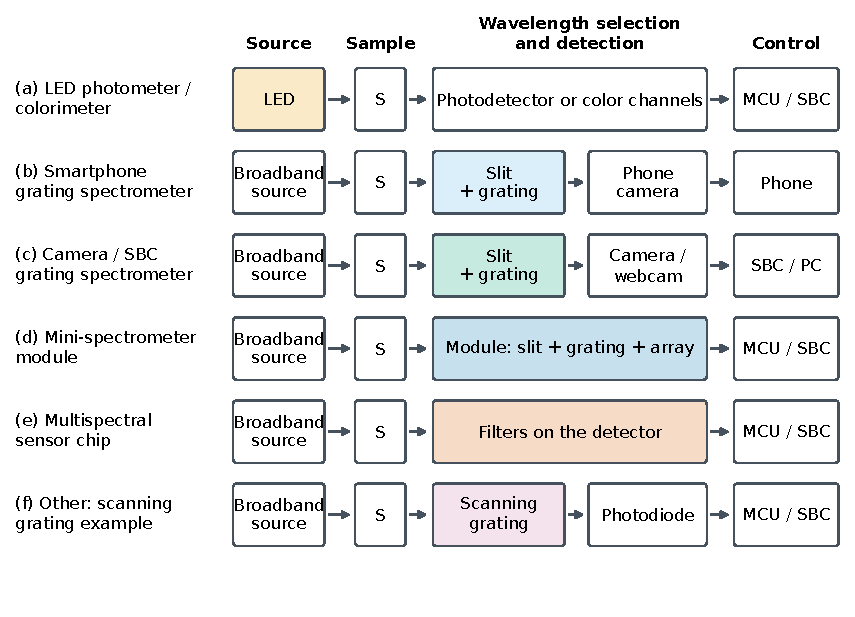
\includegraphics[width=\linewidth, draft=false]{architectures.pdf}

\caption{\FigureCaptionTwo}\label{fig:archschem}
\end{figure}

\subsection{LED photometers and colorimeters}

Instruments built around LEDs keep the optics to a bare minimum for a well-defined assay. The LED is paired with a photodiode,\citep{prairie2020accurate,glotz2018design} a phototransistor, a light-to-frequency converter, or an ambient-light sensor.\citep{nonno2022portuino,wittbrodt2015open,cirrone2025low} RGB sensors\citep{morais2015low,dewantara2023low,fernandes2023portable} and cameras without gratings\citep{tonelli2021sensing,chang2012smartphone} can serve as detectors instead. Because the emitters are interchangeable, a single instrument can handle several assays,\citep{jesus2025modular,konnel2025low} and reported applications run from UV protein measurements through visible-range chemistry to NIR screening of fuels.\citep{poh2021spectrophotometer,prairie2020accurate,dantas2017inexpensive} By combining absorbances at selected wavelengths, a six-channel LED/photodiode instrument detected and quantified synthetic hemozoin in diluted blood.\citep{catarino2020portable}

Calibration can absorb differences in sensitivity between instruments. Two LED units measured iron with sensitivities of 0.136--0.169~L/mg, compared with 0.165--0.180~L/mg for commercial instruments. Relative to the reference instruments, the reported mean sensitivities were 87.7\%, 65.2\%, and 67.0\% for iron, manganese, and fluoride, and yet recoveries in calibration checks were 98.3--104.0\%.\citep{prairie2020accurate} Selectivity is another matter: it still depends on the reagent chemistry, and on the sample matrix when absorption bands overlap.\citep{clippard2016construction,jesus2025modular,cirrone2025low}

Wavelength claims call for particular care when emitters are mixed. Combining red, green, and blue light can reproduce a color, but it does not make a monochromatic source; one assay reported at 412~nm was run on a device whose shortest emission peak lay at 458~nm.\citep{kerestes2023affordable}

\subsection{Smartphone grating spectrometers}

Phone attachments add a slit, a sample holder, and a grating to the phone camera. The grating may be a film, a piece of DVD, or a molded grating--lens element.\citep{grasse2015teaching,wang2016smartphone,zhang2016g} Alternatively, the phone can control a separate camera, which offers another route to raw data.\citep{edwards2017smartphone} Spectral coverage depends on both the illumination and the detector: a build using the phone's flash worked at 430--650~nm,\citep{wang2016smartphoneb} while an attachment with a separate camera covered 400--1000~nm with a resolution of about 5~nm.\citep{edwards2017smartphone}

Measured line widths ranged from about 0.5~nm in the narrow-slit papercraft design to 4~nm in another attachment.\citep{ju2020fabrication,markvart2020continuous} The values near 10~nm quoted for simpler builds were estimates or manufacturer specifications, not measurements.\citep{nguyen2025portable,silva2022smartphone} More elaborate optics can do several things at once. A concave blazed grating that both focused and dispersed the light, used for plasmonic sensing, achieved a measured line width of 1.075~nm with a sampling of 0.25~nm per pixel.\citep{lo2019concave} A prism-coupled evanescent-wave sensor reported a sampling of 0.305~nm per pixel, but no measured line width.\citep{dutta2014evanescent}

Acquiring several channels in parallel helps with both throughput and referencing. Dual-beam designs record sample and reference together,\citep{bogucki2019d,feng2021open} an eight-channel reader imaged the wells of an enzyme-linked immunosorbent assay (ELISA) simultaneously,\citep{wang2018ultra} and crossed gratings measured four cuvettes at once.\citep{biswas2022simultaneous} Opposite diffraction orders have also been put to use for simultaneous referencing and for repeated measurements of pH buffers.\citep{biswas2020multichannel} Optical fibers and separate cameras give more freedom in how these assemblies are mounted.\citep{long2017multimode,woodburn2019analysis,edwards2017smartphone}

The response, however, stays sensitive to the particular phone and its settings. Apparent absorptivities of permanganate came out two to four times lower than laboratory values,\citep{bruininks2022inexpensive} whereas a separately calibrated phone instrument measured 10.6~\textmu M tartrazine in a soft drink with a reference value of 10.5~\textmu M.\citep{nguyen2025portable} Reattaching the device, changing camera settings, or processing the images differently can each shift the wavelength and intensity response.\citep{markvart2020continuous,vidal2021use,matinrad2020systematic} Referencing compensates for signal variations, and light-tight construction keeps unwanted light out.\citep{bogucki2019d,nguyen2025portable,feng2021open}

\subsection{Camera and single-board-computer grating spectrometers}

A dedicated camera assembly gives more control over mounting and acquisition than a phone does. The family is small: two publications describe the PiSpec and two describe visible-range designs. The PiSpec acquires raw UV data with a modified Raspberry Pi camera, crossed Czerny--Turner optics, and a 30~\textmu m slit, and covers 280--340~nm with an FWHM of about 1~nm.\citep{wilkes2017low,wilkes2019pispec}

Ten repeated retrievals of an SO$_2$ calibration cell gave 1257\,$\pm$\,58~ppm\,$\cdot$\,m, against 1184\,$\pm$\,30~ppm\,$\cdot$\,m for a commercial spectrometer (mean\,$\pm$\,standard deviation, SD); the PiSpec needed longer exposures and its results varied more.\citep{wilkes2017low,wilkes2019pispec} When it was later deployed at Masaya volcano, its thermal drift and stray light were characterized as well.\citep{wilkes2019pispec}

For visible-range teaching, a USB camera combined with the grating from a jewelry spectroscope and a 1~mm slit gave a linear permanganate response at 540~nm between 0.05 and 0.5~mM.\citep{delmonache2025multipurpose} A webcam--DVD instrument with a resolution of about 5~nm reported 100\% accuracy in five-fold classification and a test $R^2$ of 0.9978 when predicting the syrup fraction of prepared honey mixtures.\citep{suhendar2025webcam} These last results evaluate fitted prediction models. How closely such instruments reproduce absorbance itself is a question we take up later with systems B and C.

\subsection{Mini-spectrometer modules}

Integrated modules take care of the optical assembly and leave the builder to supply illumination, sample coupling, and readout. Instruments based on the C12880MA have been used for cuvette assays, field analysis, radiometry, and reflectance,\citep{laganovska2020portable,bulusu2024technical,tunens2024optical,troscianko2023osprad,jechow2024characterizing} including measurements on leaves.\citep{leccisi2025low} With white-LED illumination, one cuvette instrument read vitamin B12 absorbance about 5--10\% below a commercial reference, with intra-day relative SDs of 1.90\% and 1.52\%, respectively.\citep{laganovska2020portable} When the same instrument was adapted for automated nitrate analysis, it was evaluated in the field against laboratory measurements; one highly concentrated sample changed color and returned a falsely low result.\citep{bulusu2024technical}

Factory alignment does not do away with the need for characterization. Measurements on these modules revealed wavelength offsets, stray light, and nonlinearity, on top of their finite bandwidth.\citep{hotra2022investigation,jechow2024characterizing,firago2022diffuse,troscianko2023osprad} The family also includes a microelectromechanical-systems (MEMS) Fabry--Perot device operating at 1100--1350~nm, used to predict sugars and acids in grape must against high-performance liquid chromatography (HPLC).\citep{krause2021smartspectrometer}

\subsection{Multispectral sensor chips}

Multispectral chips place wavelength selection and detection on the same device. Examples include the AS726x and AS734x sensors,\citep{lopin2025evaluation,yu2023open} the 18-band AS7265x spanning 410--940~nm,\citep{tran2020portable} and a 16-pixel InGaAs device covering 850--1700~nm.\citep{ou2022spectral} They have been used for predictions from reflectance,\citep{sutherland2024synchronising,noguera2022new} for absorbance measurements in cuvettes,\citep{liao2020portable,srivastava2021ultra,yu2023open,daurai2023comparison} and for reagent-coated paper assays.\citep{palekar2025microfluidic}

How they compare with full-spectrum instruments depends on the sample and the model. With 48 prediction spectra, acquired at two positions on each apple, partial least squares (PLS) regression gave $R^2_p=0.852$ and a root-mean-square error of prediction of 0.416~$^\circ$Brix with the AS7265x, compared with 0.876 and 0.398~$^\circ$Brix with a USB2000+ spectrometer (Ocean Optics).\citep{tran2020portable} On 250 corn ears of a single variety, the selected PLS workflows for the C12880MA, AS7421, and AS7265x reached test $R^2$ values of 0.91, 0.88, and 0.86, although the three sensors covered different spectral ranges and were paired with different preprocessing.\citep{himawan2026comparative}

More channels do not necessarily give better predictions. On narrow rice leaves, the six-channel AS7262 achieved a higher validation $R^2$ than the 18-channel AS7265x, which the authors put down to the separate apertures of the latter.\citep{lopin2025evaluation} Absorption outside the measured range also limited models for fruit and leaves.\citep{cano2024ataulfo,habibullah2020cost} By the same token, reconstructing a continuous spectrum from broad channels depends on the training data and on knowing the real channel responses.\citep{moralesguerra2026low,dolgalev2025development}

Chemical assays show how much response correction matters. In 43 wines, an AS7341 glucose/fructose assay gave a Passing--Bablok slope of 0.937 (95\% confidence interval 0.853--1.007) against a Cary~60 spectrophotometer (Agilent Technologies) used with a different kit, and the chip's clear channel had to be linearized at 340~nm above roughly one absorbance unit.\citep{tonelli2025portable} An AS7341 indicator array told apart similar acids that RGB data from a scanner could not,\citep{conrado2025beyond} whereas a canopy sensor combined high $R^2$ values against the reference (0.968--0.987) with slopes between 0.81 and 1.55.\citep{haryani2026evaluation}

Other studies report quantitative properties and color indices,\citep{sulistyo2021handheld,khairani2024rapid} adulteration or sample classes,\citep{rahmawati2024development,durgun2024real,gund2026development} separation by principal component analysis (PCA),\citep{wardana2025portable} and labels for origin, maturity, or treatment.\citep{habibullah2020low,sagita2025rapid,wrdana2025classification} Each of these outputs has to be judged against its own target. Moving a model to another instrument is harder still, because models are often tied to one unit\citep{stevens2024low} and change with gain, integration time, or diffuser.\citep{besozzi2026flexible,klueppel2026environmental}

\subsection{Other designs}

Some instruments replace the array detector with a mechanical scan, which then requires an angle calibration.\citep{gonzalez2020development,zainurin2023developing,hosker2017demonstrating} A scanner with a DVD grating covered 400--700~nm in steps of 1.52~nm; its absorbances differed from those of a Cary~60 by 0--12.84\% for coumarin and by 0.52--4.14\% in a mercury-ion assay.\citep{gonzalez2020development} Brick-built and optical-breadboard instruments let students see scanning and alignment at work,\citep{bougotrobin2016optimization,davis2018open} although stray light lowered the calibration slope of the unenclosed breadboard.\citep{davis2018open}

Other designs try out new approaches to fabrication or detection. In a 500--700~nm instrument with printed lenses and a prism, a filter with a nominal width of 10~nm appeared about 18~nm wide, a measure of how much the assembly broadened the band.\citep{berglund2022enabling} A UV instrument converted transmitted light at 205~nm into scintillator fluorescence that a camera could pick up; its sensitivity to nitrate was 27\% lower than that of the reference with a bandpass filter, and 85\% lower without one.\citep{booysen2021water}

\subsection{Choosing an architecture}

Choosing an architecture starts from the spectral information the measurement needs and from the geometry of the sample. Fixed bands are sufficient for well-defined assays, whereas resolved spectra reveal spectral structure and unexpected absorbers. Custom gratings give full control of the optics, integrated modules save alignment work, and multispectral chips offer compact measurements at selected bands. Which of these is appropriate comes down to whether it can meet the measurement requirement with the construction and calibration resources available.
\FloatBarrier

\section{Calibration and validation practices}\label{sec:validation}

Calibration ties the instrument signal to the quantity of interest; validation asks whether that link is good enough for a stated purpose.\citep{jcgm2012vim,eurachem2014fitness} To tell which of the two a study actually reports, one needs to know what was measured, which samples went into the calibration fit, and how performance was judged afterwards.

\subsection{Wavelength assignment and verification}

To assign wavelengths to pixels or scan positions, one needs known spectral features spread across the working range. In the studies we reviewed, these were lamp lines and lasers checked against laboratory spectra;\citep{long2014smartphone,woodburn2019analysis} nominal laser wavelengths on their own may not be accurate enough.\citep{vidal2021use} Two features are enough to define a linear mapping, but checking its residuals between and beyond them takes more.

With fixed bands, the relevant quantity is the combined response of source, optics, and detector. When channels were measured with a monochromator, they departed from their specifications,\citep{dolgalev2025development,besozzi2026flexible} and grating modules showed offsets at laser lines.\citep{hotra2022investigation,firago2022diffuse} The wavelength scale can also move later on, when the device is reattached, warms up, or changes temperature.\citep{zhang2016g,markvart2020continuous,wilkes2019pispec}

\subsection{Photometric calibration and prediction}

Absorbance is the base-10 logarithm of the ratio between the dark-corrected blank and sample intensities, a ratio that exposure, gain, nonlinear processing, and stray light can all distort.\citep{feng2021open,tonelli2021sensing,nguyen2025portable} Broadly, the calibrations we found do one of three jobs.

The first is response correction, in which the instrument itself is characterized through dark subtraction, linearization, and correction of its spectral sensitivity. A correction of this kind may only apply to one exposure setting or one sensor unit,\citep{hotra2022investigation,troscianko2023osprad,firago2022diffuse} and it is valid only for the source, model, and range in which it was established. The second job, analyte calibration, relates standards to concentration. Once calibrated, instruments with different response slopes can return comparable concentrations; residuals and curvature tests then tell whether the model fits.\citep{prairie2020accurate} Logistic or power models call for an explicit selection procedure,\citep{long2014smartphone,nonno2022portuino} and if the optical paths differ, the normalization must be justified or the comparison moved to the concentration scale.\citep{silva2022smartphone}

The third is multivariate prediction, which maps channel signals onto properties or labels.\citep{tran2020portable,kilic2018single} Such a model can only be interpreted if the preprocessing, the predictors, the model complexity, the tuning, and the number of independent physical samples are known. In the devices we reviewed, a new unit or sensor package meant a new calibration,\citep{stevens2024low,klueppel2026environmental} and transfer benchmarks run on public datasets said nothing about transfer for the authors' own instrument.\citep{krause2021smartspectrometer}

\subsection{Validation design and reference comparisons}

Repeated readings speak to repeatability; new samples, days, batches, and units test the instrument under progressively broader conditions. If a correction and its error come from the same spectra, as in one reflectance study, we still do not know how the instrument does on new samples.\citep{perezavila2024assessment} An assay can also be evaluated with independently prepared control samples, without any formal split into training and test sets.\citep{konnel2025low} With data-driven models, preprocessing, fitting, and tuning have to stay inside the training data, and repeated spectra of one physical sample have to stay together. Nested cross-validation keeps tuning apart from error estimation,\citep{varma2006bias} and one leaf study paired it with grouping by sample.\citep{lopin2025evaluation}

Comparing an instrument with a reference calls for paired evaluation samples and some account of the reference's own uncertainty.\citep{bland1986statistical} Fitting slopes or detection limits separately on each instrument does not show how individual measurements differ.\citep{wittbrodt2015open,grasse2015teaching,bruininks2022inexpensive} Genuine paired comparisons in the literature include unknown dye mixtures\citep{clippard2016construction} and field water subsamples analyzed independently.\citep{bulusu2024technical} If the two instruments rely on different reagents or sample preparation, as with wine assays run on different kits, what is being compared is two complete analytical methods.\citep{tonelli2025portable} The target needs to be explicit as well. One hydroponic instrument was calibrated against the volume of nutrient solution added but evaluated against conductivity in use, so its statistics refer to two different quantities.\citep{stevens2024low}

\subsection{Reading performance measures}

Table~\ref{tab:metricguide} sets out what each common performance measure is for, gives examples from the reviewed studies, and lists what a reader needs in order to interpret it. RMSE and MAE stand for root-mean-square and mean absolute error; SD, RSD, and CV for standard deviation, relative standard deviation, and coefficient of variation. Because the examples come from studies with different targets, they should not be read as a ranking.

A calibration $R^2$ is not a test of linearity,\citep{prairie2020accurate} and it cannot stand in for errors given in the units of the target over the relevant range of samples.\citep{cirrone2026analytical} With paired measurements, Bland--Altman limits describe how widely the differences spread. They should be weighed against a tolerance set by the application, bearing in mind their own uncertainty and any dependence on signal level. A mean bias that is not statistically significant does not, by itself, show that agreement is acceptable, and neither does a large fraction of points falling inside the estimated limits.\citep{bland1986statistical}

\begingroup
\setlength{\tabcolsep}{4pt}
\begin{xltabular}{\textwidth}{@{}>{\raggedright\arraybackslash}p{.17\textwidth} >{\raggedright\arraybackslash}X >{\raggedright\arraybackslash}X@{}}
\caption{Performance measures and their interpretation}\label{tab:metricguide}\\
\toprule
Measure & Meaning and examples from reviewed studies & Context needed for interpretation \\
\midrule
\endfirsthead
\multicolumn{3}{l}{Table \thetable{} (continued)} \\
\toprule
Measure & Meaning and examples from reviewed studies & Context needed for interpretation \\
\midrule
\endhead
$R^2$ & Calibration fit in chemical assays;\citep{laganovska2020portable} predictive performance for fruit soluble solids.\citep{tran2020portable} & Calculation method; calibration or evaluation set; sample number and range; not a test of linearity or agreement. \\
Detection or quantification limit & Low-level capability: vitamin B12, phosphate, and peroxide assays;\citep{laganovska2020portable} glucose/fructose assay.\citep{tonelli2025portable} & Definition, noise estimate, calibration model, units, and experimental verification near the claimed limit. \\
Prediction RMSE or MAE & Error in target units: nitrate concentration (RMSE);\citep{bulusu2024technical} leaf chlorophyll content (MAE).\citep{lopin2025evaluation} & Evaluation samples, range, and split procedure; training errors distinguished from errors on new samples. \\
Mean bias & Average paired difference from a reference: wine glucose/fructose measurements.\citep{tonelli2025portable} & Sign convention, units, and uncertainty; a small mean bias can conceal large individual differences. \\
Bland--Altman limits & Spread of paired differences: immunoassays\citep{long2014smartphone} and serum biochemical assays.\citep{luo2021smartphone} & Difference plot, assumptions, uncertainty, and application-specific acceptance limits. \\
SD, RSD or CV & Dispersion of repeated measurements: within- and between-day assay results;\citep{laganovska2020portable} repeated glucose/fructose measurements.\citep{tonelli2025portable} & Number and type of repetitions, repositioning, and operating conditions; repeatability does not establish low bias. \\
Classification accuracy & Fraction of labels correctly predicted: fuel adulteration\citep{dantas2017inexpensive} and plant nitrogen-status classes.\citep{habibullah2020low} & Class counts, confusion matrix, decision rule, and separation of training and evaluation samples. \\
\bottomrule

\end{xltabular}
\endgroup

A detection limit means little without the way it was derived (blank variation, control charts, or regression) and without low-concentration measurements that back it up.\citep{silva2022smartphone,prairie2020accurate,konnel2025low} When detection rests on a model prediction, the decision threshold has to carry the uncertainty of that prediction.\citep{suhendar2025webcam} In the same way, scaled performance measures only make sense with a common target and reference.\citep{martinezavino2021scaling}

\subsection{Characteristics of the analyzed studies}

Table~\ref{tab:valpractice} summarizes what the analyzed studies documented, first by hardware family and then by principal application. Each study appears once in each part of the table, and the notes underneath define the columns. Several patterns are worth pointing out. Most studies compared their instrument with a reference, yet only about half put a number on the agreement, and fewer than half tested it on samples that had not been used for calibration. Real matrices and held-out samples were most common in the studies on multispectral chips, many of which built prediction models for agricultural products. Repeatability, by contrast, was reported far more often for LED photometers than for any other family. The last row of the first part shows, for comparison, how our systems A, B, and C (described in the next section) fare against the same criteria.

\Needspace{24\baselineskip}
\begingroup
\small
\setlength{\tabcolsep}{4pt}
\begin{xltabular}{\textwidth}{@{}>{\raggedright\arraybackslash}X rrrrrrrr@{}}
\caption{What the analyzed studies documented, by hardware family and by principal application}\label{tab:valpractice}\\
\toprule
 & $n$ & Reference & Quantified & Held-out & \shortstack[r]{Real\\matrix} & \shortstack[r]{Repeat-\\ability} & Cost & \shortstack[r]{Open\\files} \\
\midrule
\endfirsthead
\multicolumn{9}{l}{Table \thetable{} (continued)} \\
\toprule
 & $n$ & Reference & Quantified & Held-out & \shortstack[r]{Real\\matrix} & \shortstack[r]{Repeat-\\ability} & Cost & \shortstack[r]{Open\\files} \\
\midrule
\endhead
\multicolumn{9}{l}{\textit{By hardware family}} \\
LED & 28 & 22 & 15 & 14 & 15 & 23 & 17 & 9 \\
Phone & 29 & 23 & 16 & 10 & 11 & 14 & 17 & 7 \\
Camera/SBC & 4 & 3 & 2 & 1 & 2 & 2 & 4 & 1 \\
Module & 9 & 8 & 3 & 3 & 4 & 2 & 5 & 5 \\
Chip & 34 & 25 & 21 & 22 & 27 & 9 & 12 & 6 \\
Other & 7 & 7 & 3 & 1 & 2 & 2 & 1 & 2 \\
\midrule
All studies & 111 & 88 & 60 & 51 & 61 & 52 & 56 & 30 \\
Systems A--C (this work) & --- & yes & yes & yes & no & yes & yes & yes \\
\midrule
\multicolumn{9}{l}{\textit{By principal application}} \\
Environment & 31 & 30 & 22 & 14 & 18 & 23 & 19 & 10 \\
Agriculture/food & 31 & 21 & 20 & 23 & 29 & 5 & 11 & 4 \\
Biomedical & 17 & 14 & 8 & 7 & 9 & 12 & 11 & 2 \\
Education/citizen science & 20 & 14 & 5 & 4 & 3 & 6 & 11 & 14 \\
Instrumentation/industry & 12 & 9 & 5 & 3 & 2 & 6 & 4 & 0 \\
\bottomrule
\end{xltabular}
\vspace{-6pt}
\noindent\begin{minipage}{\textwidth}\footnotesize\raggedright
Entries are numbers of studies documenting each characteristic, and $n$ is the number of studies in the group. A study can contribute to several columns, so the columns should not be added, and a characteristic that was not documented should not be read as proven absent.
\textit{Reference}: comparison with a reference instrument or an accepted method, qualitative or quantitative (unrelated to $R^2$).
\textit{Quantified}: a numerical comparison with that reference, such as errors, correlations, separately fitted sensitivities, or peak positions; it shows that agreement was reported, not that it was acceptable.
\textit{Held-out}: evaluation on samples not used for calibration fitting, with or without a formal test set.
\textit{Real matrix}: measurements on real samples rather than prepared standards only.
\textit{Repeatability}: repeatability given numerically or as error bars explicitly based on repeated measurements.
\textit{Cost}: a numerical cost total that can be plotted in Figure~\ref{fig:costres}; lists of component prices alone are not counted.
\textit{Open files}: shared design files or code, without checking licensing or successful rebuilding.
For systems A--C, the validation dyes were kept out of fitting and model selection, but prepared dye solutions do not count as real matrices. The coding of each study is available from the authors on reasonable request.
\end{minipage}
\endgroup
\FloatBarrier

\section{Systems A, B, and C under a common protocol}\label{sec:case}

Because the studies reviewed above were evaluated with different samples, references, and metrics, it is hard to say how much of the reported differences comes from the hardware and how much from the way each instrument was tested. To see what a common protocol reveals, we measured three inexpensive instruments side by side, using the same dye solutions, cuvettes, light source, and laboratory reference for all of them.

There were several reasons for choosing these three instruments. Together they represent two of the most widespread routes in the literature: a multispectral sensor chip, the largest hardware family in Table~\ref{tab:valpractice}, and a camera-based grating spectrometer, the approach shared by the smartphone and camera families. All three cost less than \euro{}220, which places them well within the price range of the instruments reviewed. They also illustrate three ways in which a user can obtain such an instrument: building it around an open sensor board (system A), assembling it from a commercial pocket spectroscope and a single-board computer running open software (system B), or buying it ready-made (system C). Finally, the three instruments were available to us through our work on low-cost tools for monitoring water quality, which is the kind of application such devices are intended for.

System A uses an AS7265x multispectral sensor, system B a Raspberry Pi camera behind a pocket spectroscope, and system C a Little Garden webcam spectrometer. For each, we evaluated absorbance agreement with the reference, repeatability, calibration size, and cost.

\subsection{Materials and methods}\label{sec2}

The reference instrument was a single-beam Genesys~30 spectrophotometer (Thermo Fisher Scientific; 325--1100~nm). Its specified bandwidth is 5~nm, its wavelength accuracy $\pm$2~nm, and its photometric accuracy $\pm$0.002 absorbance units between 0 and 0.3 and 0.5\% of the reading between 0.301 and 2.5.\citep{thermoGenesys30}

\subsubsection{Systems A, B, and C}\label{subsec2.1}

Figure~\ref{fig:systems} shows the three systems.

\begin{figure}[!htbp]
\centering
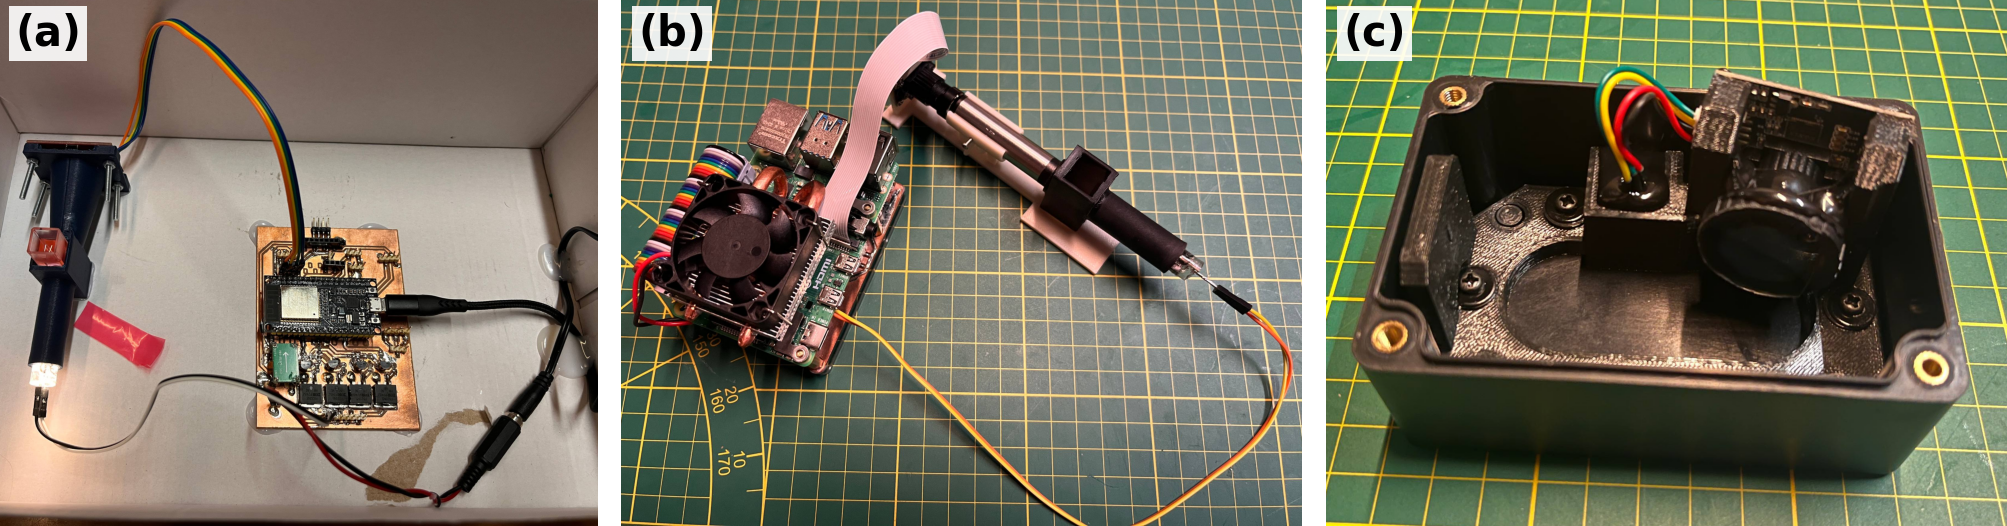
\includegraphics[width=\linewidth, draft=false]{systems.png}

\caption{\FigureCaptionThree}\label{fig:systems}
\end{figure}

System A is built around the SparkFun Triad AS7265x multispectral sensor board (SparkFun Electronics). The board integrates three CMOS devices (AS72651, AS72652, and AS72653; ams OSRAM) and provides 18 spectral channels between 410 and 940~nm. Interference filters deposited on the sensor define the channels, with a nominal FWHM of about 20~nm,\citep{ams2018as7265x} so no external dispersive optics are required. We disabled the built-in LEDs so that the sensor could be used with the external source, and mounted the assembly on a custom 3D-printed structure. An ESP32 microcontroller handled communication and acquisition, and the acquisition software averaged ten consecutive measurements per reading. Absorbance was calculated as the base-10 logarithm of the ratio between blank and sample intensities.

System B is an imaging spectrometer: a Raspberry Pi camera records the output of a commercial pocket spectroscope fitted with a transmission diffraction grating (Pocket Spectroscope, Paton Hawksley Education).\citep{patonPocket} A 12~mm M12 lens focuses the spectrum onto the sensor, and a Raspberry Pi 4B single-board computer (Raspberry Pi Ltd) controls acquisition. Camera and spectroscope were mounted on a custom 3D-printed structure. Spectra were acquired and processed with PySpectrometer2,\citep{wrightPySpectrometer2} which extracts the spectrum by vertical averaging and supports wavelength calibration with several reference points.

System C is the Little Garden spectrometer, a commercial low-cost instrument. Inside a 3D-printed enclosure that connects to a computer by USB, it combines a modified webcam, with the Bayer filter removed to increase sensitivity, and a grating cut from a DVD. Spectra were acquired with the Theremino Spectrometer software\citep{thereminoSpectrometer} at a resolution of 1920\,$\times$\,1080 pixels. Before each measurement, we adjusted the vertical region of interest by hand so as to capture the spectrum while keeping the background low.

The three systems shared the same 10~W halogen lamp, but their holders and collection optics differed, so their complete optical paths were not identical.

\subsubsection{Calibration}\label{subsec2.2}

\paragraph{Preparation of the dye solutions}\label{subsubsec2.2.1}

Each of the eleven solutions contained one drop of a commercial food dye in 10~mL of distilled water (twelve-color set, 6~mL per bottle; Amazon ASIN B08X6FMHKP). The manufacturer does not disclose the colorants or their concentrations, so we identify the dyes by their commercial names and reference spectra. Eight dyes (grape, lemon, lime, navy, orange, pink, rose, and teal) supplied the calibration data, while the blue, green, and red dyes were kept out of fitting and model selection and reserved for validation. Validation therefore concerns new solutions from the same family of colorants, whose absorption bands may overlap (blue and teal both peak near 630~nm). The lemon and rose solutions reached absorbances of 2.85 and 2.68, beyond the range over which the photometric accuracy of the reference is specified; these values were retained in the calibration fits. Nine of the reference spectra are shown in Figure~\ref{fig:dyes}; orange and pink are omitted.

\begin{figure}[!htbp]
\centering
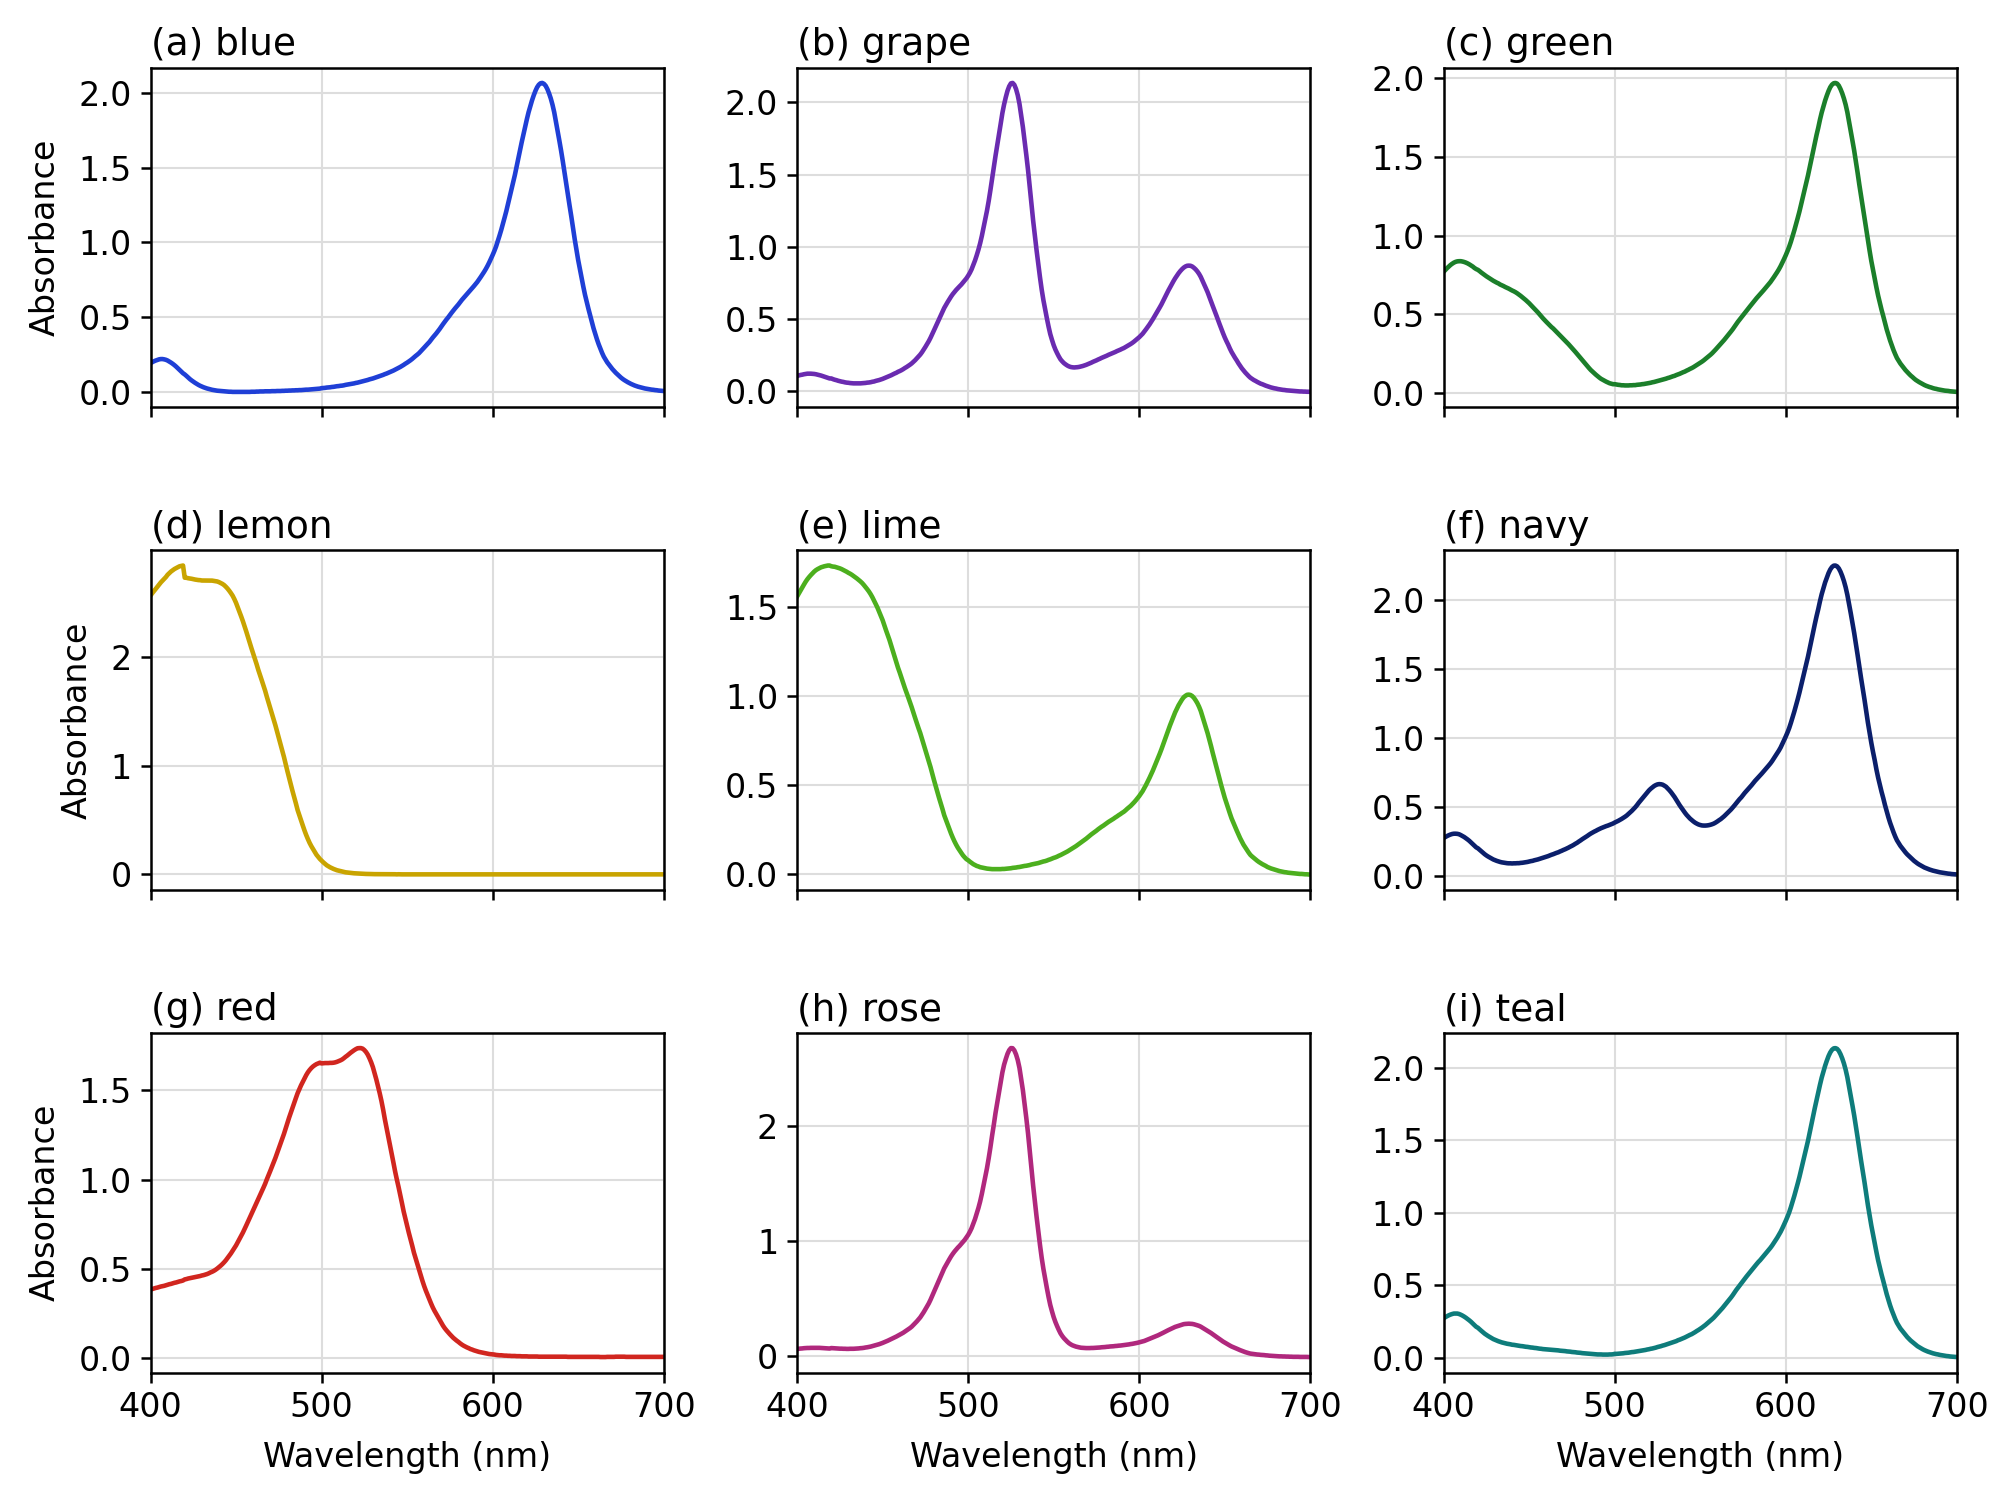
\includegraphics[width=\linewidth, draft=false]{commercial.png}

\caption{\FigureCaptionFour}\label{fig:dyes}
\end{figure}

\paragraph{Wavelength calibration}\label{subsubsec2.2.2}

For system A we relied on the nominal channel centers and did not independently verify the position or response of the channels. For the two imaging systems, mercury lines defined the mapping from pixels to wavelengths: a cubic polynomial through 404.7, 435.8, 546.1, and 577.0~nm for system B, and a straight line through 435.8 and 546.1~nm for system C. A cubic through four points and a line through two leave no residual degrees of freedom, and we did not measure any additional line to check either mapping.

\paragraph{Absorbance calibration}\label{subsubsec2.2.3}

Measured absorbance $s$ was related to reference absorbance $A_{\text{ref}}$ through a wavelength-dependent gain and offset:
\begin{equation}\label{eq:cal}
A_{\text{ref}} \;=\; a_1(\lambda)\, s \;+\; a_0(\lambda)
\end{equation}
where $a_1$ is the gain, $a_0$ the offset, and $\lambda$ the wavelength. Before fitting, measured absorbances above 5 were excluded automatically, and calibration required at least three valid dye pairs at each wavelength. Systems A and C used eight calibration pairs throughout. System B used seven pairs below 420~nm, where the navy dye measurements exceeded the threshold, and eight at the remaining wavelengths. Adding a second-order term in $s$ to Eq.~\ref{eq:cal} did not improve leave-one-dye-out prediction within the eight calibration dyes and was unstable for system B, so we kept the first-order model.

A single gain and offset for all wavelengths could not reproduce the reference. For systems B and C, we therefore expanded $a_1(\lambda)$ and $a_0(\lambda)$ in an orthogonal polynomial basis of normalized wavelength, of degree 18 for B and 8 for C, and fitted them jointly by least squares across all calibration dyes and wavelengths. Both degrees were selected by leave-one-dye-out cross-validation within the eight calibration dyes, so the validation dyes stayed outside model selection. The resulting smooth surfaces can be evaluated anywhere in the calibrated range. The discrete channels of system A were fitted separately, with two coefficients per channel, whereas systems B and C need two coefficients per term of the polynomial expansion.

\subsubsection{Validation measurements and metrics}\label{subsec2.3}

All measurements were made in 10~mm plastic cuvettes, in darkness and at an ambient temperature of 22~$^\circ$C, with blank and dark spectra acquired before each series. Each validation dye was measured 100 times on each system, with the cuvette repositioned by hand between readings.

To summarize agreement over 400--700~nm, we used the root-mean-square difference (RMSD), pooling the paired differences between calibrated and reference absorbance over all wavelengths and the three validation dyes. The squared Pearson correlation ($r^2$) was computed separately for each dye and then averaged. RMSD measures differences in absorbance units, whereas $r^2$ captures how well the spectral shapes match and is insensitive to a constant bias. System A was compared with the reference at its nominal channel centers, and systems B and C on their own wavelength grids.

For repeatability, we computed the SD of the 100 readings at each wavelength and averaged it over wavelength and over the three dyes. The pointwise coefficient of variation was $\mathrm{CV}=100\,\mathrm{SD}/\overline{A}$, where $\overline{A}$ is the mean absorbance, using only points with $\overline{A}>0.05$; these CVs were averaged over wavelength for each dye and then over the three dyes. SD thus expresses absolute dispersion, and CV dispersion relative to the mean signal. Since each reading of system A is already an average of ten sensor measurements, the repeatability results describe the acquisition procedures as they were used. We did not quantify spectral resolution, portability, ease of use, assembly time, maintenance effort, or power demand.
\FloatBarrier

\subsection{Results and discussion}\label{sec4}

Table~\ref{tab:metrics} summarizes, for each system, the agreement with the reference (RMSD and $r^2$), the spectral sampling ($n_\lambda$, the number of wavelengths per dye), the size of the calibration ($N_c$, the total number of fitted coefficients), and the repeatability (SD and CV), all over 400--700~nm and the three validation dyes. The pooled comparisons contain 33, 903, and 1710 wavelength--dye pairs for systems A, B, and C; because neighboring spectral points are correlated, these numbers are not counts of independent samples.

Of the three, system B came closest to the reference in absorbance and had the smallest absolute SD. System C had a slightly higher RMSD and greater dispersion, but needed the fewest calibration coefficients.

\begin{table}[!htbp]
\doublespacing
\caption{Performance of systems A, B, and C on the three validation dyes over 400--700~nm}\label{tab:metrics}
\centering

\begin{tabular}{lrrrrrr}
\toprule
System & RMSD & $r^{2}$ & $n_\lambda$ & $N_{c}$ & SD & CV (\%) \\
\midrule
A & 0.281 & 0.805 & 11  & 22 & 0.050 & 12.1 \\
B & 0.077 & 0.983 & 301 & 38 & 0.032 & 11.1 \\
C & 0.094 & 0.975 & 570 & 18 & 0.086 & 32.3 \\
\bottomrule
\end{tabular}

\end{table}

\begin{figure}[!htbp]
\centering
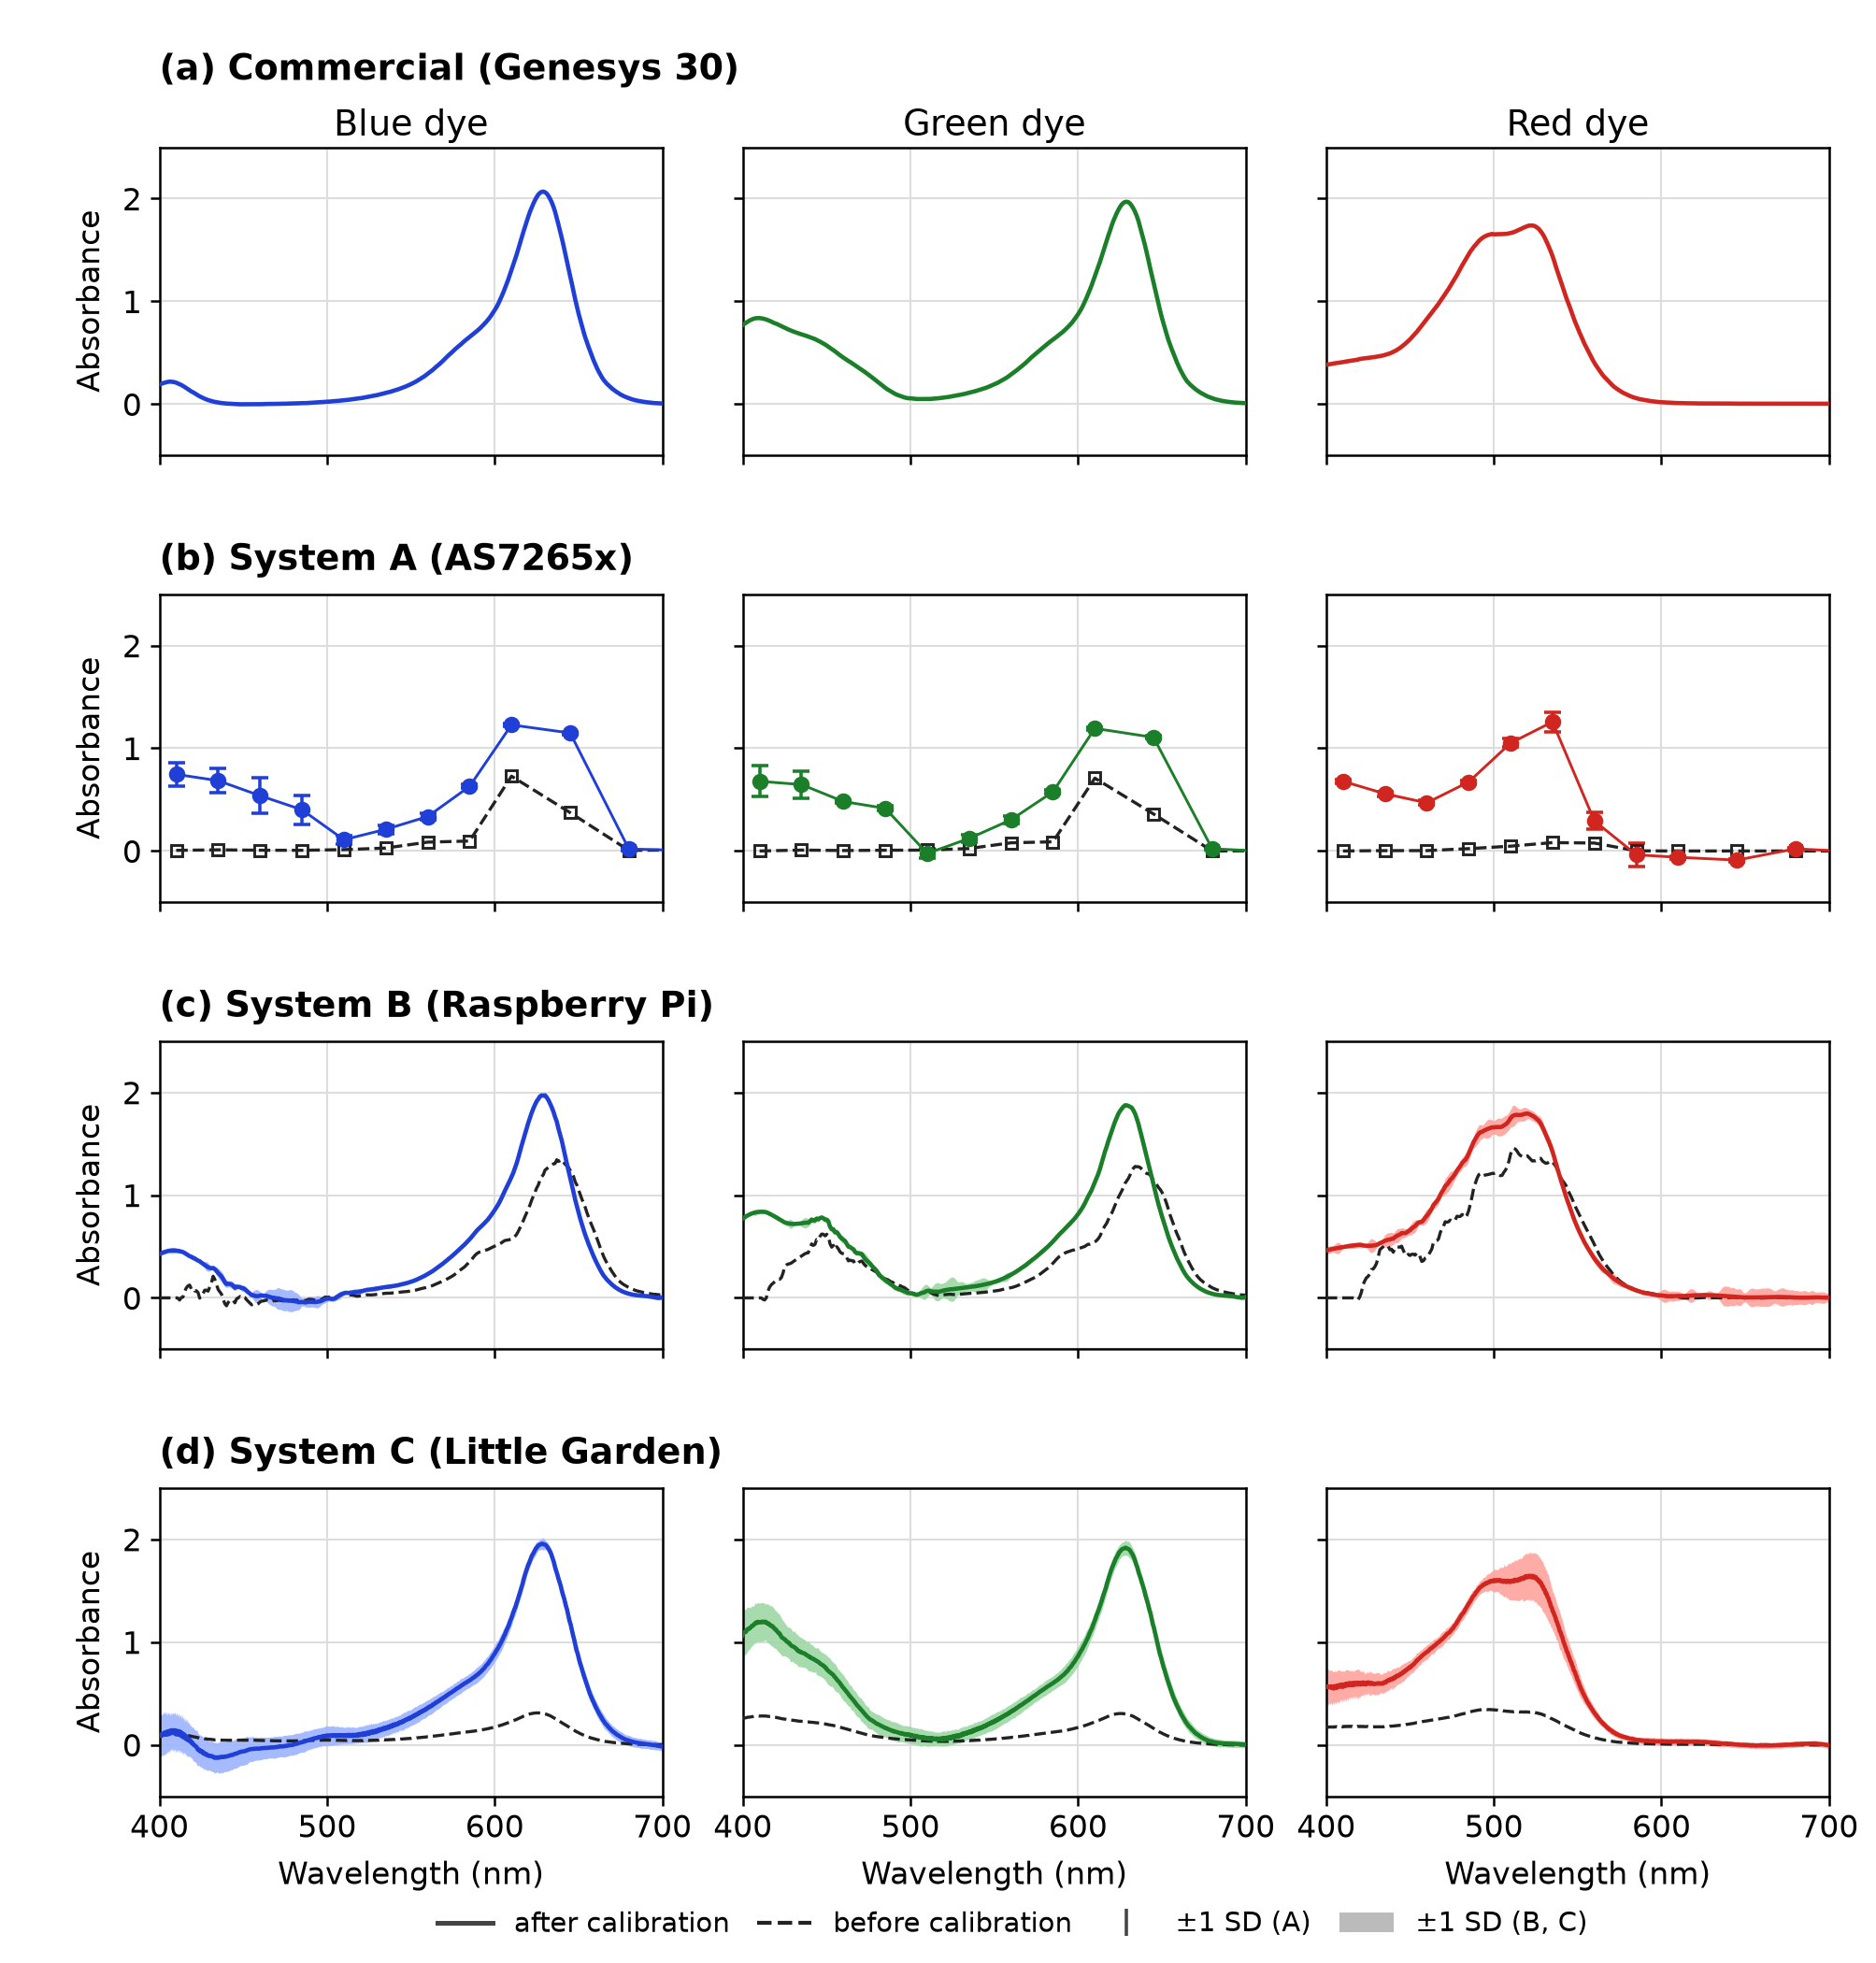
\includegraphics[width=\linewidth, draft=false]{comparison.png}

\caption{\FigureCaptionFive}\label{fig:comparison}
\end{figure}
\FloatBarrier


All three systems located the main absorption bands (Figure~\ref{fig:comparison}). Calibration stretched the initially compressed responses, above all those of systems A and C; such compression is consistent with stray light and with broad effective bandwidths, neither of which we measured. System A captured the overall shape of the spectra but missed their finer detail, while system B showed moderate noise in the blue region and weaker noise in the green. The wider shaded bands of system C reflect its larger absolute SD. Both channel bandwidth and optical coupling affect how system A compares with point values of the reference, but we were unable to separate their contributions.

In Figure~\ref{fig:map}, the points for systems B and C lie close to the identity line over most of the range, while those for system A scatter more widely. Below 480~nm, the mean absolute differences were 2.1, 2.3, and 3.4 times larger than above 480~nm for systems A, B, and C, respectively. This pattern is consistent with the weak blue output of the halogen lamp, but since the three systems share silicon detectors, cuvettes, and calibration samples, we could not isolate its contribution.

\begin{figure}[!htbp]
\centering
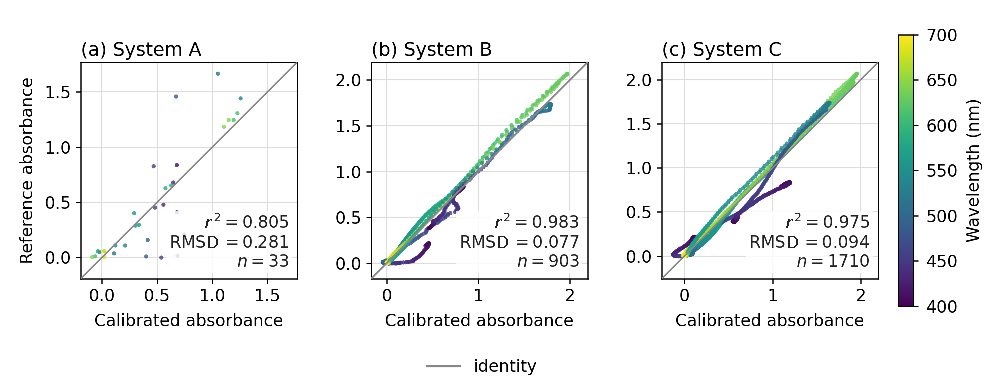
\includegraphics[width=\linewidth, draft=false]{dispersion.pdf}

\caption{\FigureCaptionSix}\label{fig:map}
\end{figure}

\subsubsection{Implementation and cost}\label{sec4.1}

System A cost \euro{}88: \euro{}65 for the sensor, \euro{}8 for the controller, \euro{}10 for the enclosure and accessories, and \euro{}5 for wiring, circuit board, and power supply. System B cost \euro{}215: \euro{}15 for the camera, \euro{}65 for the Raspberry Pi, \euro{}15 for the lens, \euro{}100 for the spectroscope, \euro{}10 for the enclosure and accessories, and \euro{}10 for wiring, circuit board, and power supply. System C was bought as a complete retail instrument for \euro{}90. None of these totals includes the shared halogen lamp, the purchase dates are not available, and the component totals for systems A and B do not cover the same items as the retail price of system C.

\subsubsection{Scope and limitations}\label{sec:caselim}

Our comparison rests on a single unit of each system and on three validation solutions from the same family of colorants as the calibration set, and two of the calibration dyes exceeded the specified photometric range of the reference. We did not measure resolution, stray light, drift, transfer between units, performance in real matrices, or detection limits. Neither the nominal filter responses nor the wavelength mappings were verified independently, and the systems are no longer available for further measurements. The results therefore apply to the units, calibrations, and acquisition settings we tested.
\FloatBarrier

\section{Applications}\label{sec:applications}

We assigned each publication to one principal application: environmental monitoring; agriculture and food; biomedical testing; education and citizen science; or instrumentation and industry (Table~\ref{tab:valpractice}). How the instruments were evaluated varied noticeably from one group to another. Environmental monitoring and agriculture and food, for instance, are equally large groups, yet repeatability was reported in most of the environmental studies and in only a handful of the agricultural ones.

\subsection{Water quality and environmental monitoring}

Water studies provide comparisons based on standards, spiked waters, and field samples. An arsenic photometer was compared with inductively coupled plasma mass spectrometry (ICP-MS) in six spiked environmental waters.\citep{awasthi2023portable} A phone instrument measured tap, spring, river, and well waters and returned 1.06~mg/L for a chlorine reference of 1.10~mg/L.\citep{sargazi2020application} In 12 river samples measured in triplicate, the mean relative differences from a Cary~60 at each site were 4.6--12.6\% for nitrate and 2.0--18.8\% for phosphate, though individual phosphate differences reached 30.9\%.\citep{cirrone2025low} In wastewater, differences of up to 26.5\% were reported, particularly near the detection limit,\citep{silva2022smartphone} and in two treated effluents the differences were 19\% and 7\%.\citep{booysen2021water}

Working in the field adds reagent delivery, fouling, and maintenance to the optical requirements. In three field tests, a solar-powered automated nitrate analyzer achieved root-mean-square errors of 0.09--0.20~mg/L NO$_3^-$-N against laboratory analyses.\citep{bulusu2024technical} Evaluations of commercial in situ probes give further context for deployments of this kind.\citep{zhu2021assessment} Volcanic SO$_2$ retrieval,\citep{wilkes2017low,wilkes2019pispec} lake reflectance,\citep{jechow2024characterizing} and radiometry of artificial light\citep{troscianko2023osprad} extend monitoring beyond aqueous assays, each with references specific to the quantity being measured.

\subsection{Agriculture and food}

Nearly all of the agriculture and food studies measured real matrices. Among the quantitative predictions were fructose in grape must against HPLC (test $R^2=0.91$),\citep{krause2021smartspectrometer} and soluble solids in grapes and fat content in olives (leave-one-out $R^2=0.70$ and 0.75).\citep{noguera2022new,aquino2022preliminary} One leaf study grouped spectra by sample and used nested model selection;\citep{lopin2025evaluation} another applied a color classifier trained on Pantone references to 16 leaves, with no independent biochemical check of how it interpreted leaf health.\citep{leccisi2025low}

A classification result means something only when the classes and the evaluation procedure are stated. One report on spice adulteration claimed an accuracy above 90\% without documenting the size of the test set or how the data were split.\citep{gund2026development} For the maturity of oil-palm fruit, test accuracies were 60\%, 80\%, and 100\% for random forests, support-vector machines, and nearest neighbors.\citep{suci2025determination} Fertilizer treatments were classified with 94.2\% accuracy in a two-class greenhouse task and 79.2\% in the field, without any direct measurement of leaf nitrogen.\citep{habibullah2020low} Classification of coffee origin and of meat,\citep{sagita2025rapid,wrdana2025classification} together with commercial handheld systems,\citep{mullermaatsch2021handheld,bec2022miniaturized} widens the range of applications, although transfer across batches, cultivars, and seasons has yet to be shown.

Light and vegetation indices are a different kind of target. A radiometer reported mean relative errors of 1.61--8.29\% for the components of photosynthetic photon flux in 77 test measurements.\citep{dolgalev2025development} A sensor for the normalized difference vegetation index (NDVI) gave $R^2=0.997$ against a hyperspectral reference on 13 laboratory targets.\citep{kitic2019new}

\subsection{Biomedical and point-of-care testing}

Roughly half of the biomedical studies used real or clinical matrices. An eight-channel phone ELISA reader agreed with the reference diagnostic calls for four autoantibody assays in 180 patient sera, although each assay had only one to nine positive samples.\citep{wang2018ultra} Another phone reader tested six analytes in 12 sera and reported correlations of 0.905--0.999 along with Bland--Altman analyses.\citep{luo2021smartphone} A reader for paper assays differed from clinical results by 1.9--10.5\% for alkaline phosphatase and 1.3--7.2\% for total protein.\citep{arunraj2024design}

Laboratory demonstrations rest on evidence of a different kind. An AS7341 paper reader was tested against commercial biochemical controls, with no documented series of patient sera.\citep{palekar2025microfluidic} A hemozoin reader was tested with synthetic hemozoin in water, in hemoglobin, and in diluted blood from healthy donors, so its sensitivity and specificity describe those assays.\citep{catarino2020portable} Preclinical measurements included fetal fibronectin standards and spiked plasma,\citep{long2017multimode} and the retrieval of absorption in tissue phantoms with a mean error of 9.2\%, against 6.1\% for a benchtop system.\citep{edwards2017smartphone} Toxicological and biochemical readers\citep{wang2016smartphone,kong2020novel,yu2023open} are also discussed in broader reviews.\citep{hussain2021smartphone,geng2017recent} Going beyond these laboratory demonstrations to establish clinical performance will require patient cohorts with enough positive cases.

\subsection{Education and citizen science}

Instruments built for teaching let students observe alignment, wavelength assignment, and Beer--Lambert behavior for themselves.\citep{gonzalezlaprea2025d,vusirikala2026bringing} Their imperfections can even become useful experiments. Camera instruments showed reduced slopes or absorptivities,\citep{grasse2015teaching,nguyen2025portable,bruininks2022inexpensive} and in one case a double-beam instrument and a commercial reference returned 0.0903~M and 0.0906~M for a copper sulfate unknown prepared at 0.1095~M.\citep{winters2021d} The close agreement between the two instruments therefore hid an error of about 17\% relative to the prepared concentration. A colorimeter evaluated on unknown binary dye mixtures was compared both with the prepared values and with a laboratory reference.\citep{clippard2016construction}

Most of the educational studies shared their files or code, but only a few measured real matrices. Dual-beam and community photometers connect teaching with environmental monitoring,\citep{feng2021open,cirrone2025low,konnel2025low} where evaluation has to cover the relevant waters, users, and operating conditions.\citep{cirrone2026analytical}

\subsection{Instrumentation and industry}

The studies in this last group deal with fuel and process analysis,\citep{dantas2017inexpensive,glotz2018design,vidal2021brand} optical characterization,\citep{berglund2022enabling,matinrad2020systematic,firago2022diffuse,hotra2022investigation,perezavila2024assessment} and fiber, evanescent-wave, plasmonic, or multichannel sensing.\citep{markvart2020continuous,dutta2014evanescent,lo2019concave,biswas2020multichannel} What they report is the measured optical response or the process target, and it should not be read as the performance of a sample-based assay.

\section{Open hardware, reproducibility, and cost}\label{sec:openhw}

Only about a quarter of the analyzed studies shared their design files or code. Those that did used GitHub, OSF, Zenodo, figshare, and design-sharing platforms,\citep{wittbrodt2015open,feng2021open,bulusu2024technical,stevens2024low,bogucki2019d,grasse2015teaching} or supplied the files with the article,\citep{prairie2020accurate,nonno2022portuino,delmonache2025multipurpose,yu2023open} in some cases including optical components that others can adapt.\citep{zhang2013open} The review of freshwater sensors likewise found that design files were rarely available.\citep{cirrone2026analytical}

Being able to download the files is only a start: reuse also depends on how complete they are and how they are licensed.\citep{wenzel2023open} EOSpec, for example, pairs MIT-licensed software with a noncommercial Creative Commons license for the remaining materials,\citep{feng2021open} and another instrument uses CERN-OHL-S for the hardware and separate terms for software and documentation.\citep{moralesguerra2026low} Files available only on request,\citep{glotz2018design,markvart2020continuous} or an application released without its source code,\citep{hosker2017demonstrating} leave far fewer routes to modifying and rebuilding an instrument.

\subsection{Rebuilding and calibration transfer}

Every rebuilt instrument needs its own evaluation of response. Two LED units differed in their sensitivity to iron, which the authors attributed to differences in component performance; source intensity and blank voltage also affected the calibration.\citep{prairie2020accurate} Five C12880MA spectroradiometers were characterized one by one, with shared corrections offered as an alternative.\citep{troscianko2023osprad} Two encapsulated AS7265x units gave mean readings of 13\,019.59 and 36\,185.52 counts for the same empty tank, and each needed its own model.\citep{stevens2024low} Switching phone models or reassembling an attachment brought further changes in response.\citep{bruininks2022inexpensive,vidal2021use}

Calibration data and processing records help to disentangle the effects of construction from those of analysis choices.\citep{troscianko2023osprad,moralesguerra2026low,stevens2023development,prairie2020accurate} The nitrate analyzer derived from the open-source C12880MA instrument shows how a shared design can be adapted and then evaluated for a new application.\citep{bulusu2024technical,laganovska2020portable} We intend the files we provide for systems A and B to be used in the same way: a rebuilt unit should be recalibrated and evaluated before use.

\subsection{Reading reported costs}

Figure~\ref{fig:costres} plots the numerical cost totals counted in Table~\ref{tab:valpractice}, with one marker per publication. Most are totals for a complete device or the sum of its components; the rest refer to phone attachments, sensor boards alone, or larger systems. The stars mark our systems A, B, and C, using component totals for A and B and the retail price for C.

Most totals were originally given in US dollars, and the rest in euros, pounds sterling, or Singapore dollars, in publications dated between 2015 and 2026. The original currencies, exclusions, and source evidence are kept in the extraction records. Since the dates of the prices were stated inconsistently, a common display currency does not imply equivalent purchasing conditions.

\begin{figure}[!htbp]
\centering
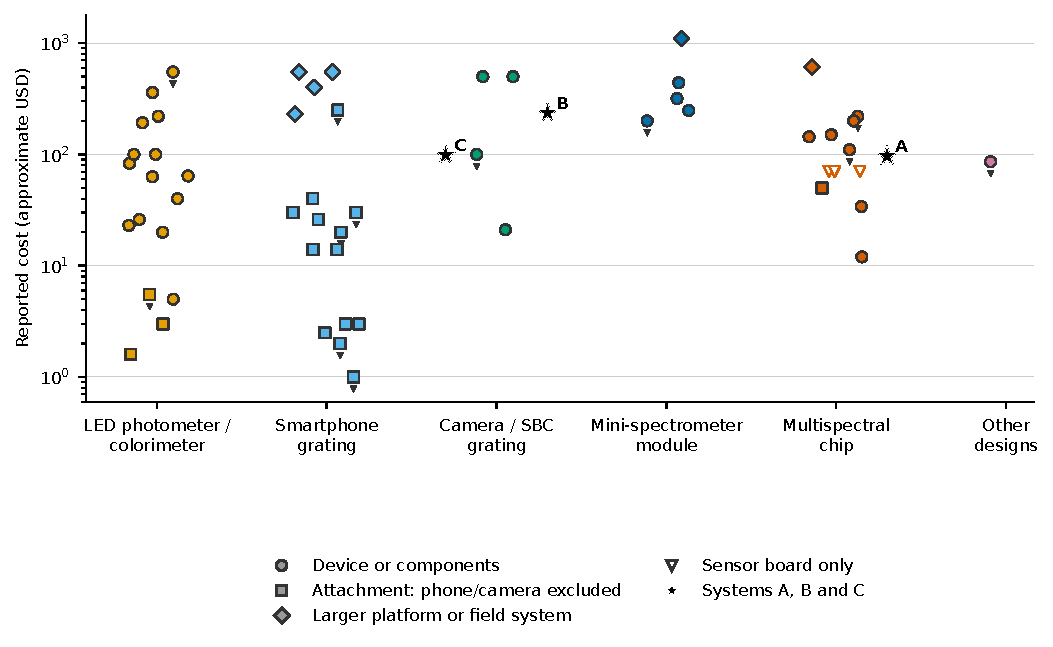
\includegraphics[width=\linewidth, draft=false]{cost_channels.pdf}
\caption{\FigureCaptionSeven}\label{fig:costres}
\end{figure}

Much of the spread comes down to what each price includes. Attachment prices leave out the phone or camera,\citep{koohkan2020fabrication,rani2021polynomial,ju2020fabrication,feng2021open} and sensor-board prices of USD~28--70 leave out the rest of the acquisition assembly.\citep{stevens2023development,stevens2024low,lopin2025evaluation} Three reports on larger systems were unclear about whether the phone was included,\citep{wang2016smartphone,long2017multimode,woodburn2019analysis} while others priced a reader together with its phone, a spectral camera, or a field analyzer.\citep{kong2020novel,sutherland2024synchronising,bulusu2024technical}

The shared designs show just how different these budgets can be: a USD~63 analog photometer,\citep{prairie2020accurate} a USD~26 freshwater photometer,\citep{cirrone2025low} the USD~30 EOSpec,\citep{feng2021open} and the EUR~225 C12880MA instrument along with its USD~1100 field adaptation.\citep{laganovska2020portable,bulusu2024technical} Teaching hardware below USD~100, a USD~50 handheld spectrometer, and a USD~144 horticultural sensor are further examples.\citep{delmonache2025multipurpose,yu2023open,moralesguerra2026low} Lists of component prices\citep{nguyen2025portable} and prices of individual printed optical mounts\citep{davis2018open} give partial information, but no instrument total that could be plotted.

Cost estimates also differ in the equipment they leave out,\citep{wang2015build} in whether they count parts only,\citep{prairie2020accurate} in whether they include reagents or fabrication,\citep{liao2020portable,habibullah2020cost} and in whether they assume manufacturing or market prices.\citep{aquino2022preliminary,kitic2019new} For an estimate to be useful to someone rebuilding the instrument, it therefore needs a dated bill of materials, a list of exclusions, the cost of assembly and calibration, and recurring expenses. These prices and channel or pixel counts are so heterogeneous that they cannot support a comparison of analytical performance per dollar.

\section{Challenges and outlook}\label{sec:outlook}

\subsection{Reporting requirements}

In Table~\ref{tab:checklist} we translate the findings of this review into reporting items that cover optical construction, measurement performance, cost, and rebuilding. The checklist extends the framework proposed for freshwater sensors\citep{cirrone2026analytical} to all six hardware families. What it asks for depends on the application; it does not assign a quality score, and it does not claim to be a consensus standard.

Each row names an item, describes the information to report, and shows how well our systems A, B, and C cover it. ``Yes'' means the information is reported here, ``Partial'' points to gaps, and ``No'' marks an assessment we did not perform. Authors can use the middle column to select what matters for their own application and to explain what they leave out.

\Needspace{12\baselineskip}
\begingroup
\setlength{\tabcolsep}{4pt}
\begin{xltabular}{\textwidth}{@{}>{\raggedright\arraybackslash}p{0.20\textwidth} >{\raggedright\arraybackslash}X >{\raggedright\arraybackslash}p{0.20\textwidth}@{}}
\caption{Reporting checklist}\label{tab:checklist}\\
\toprule
Item & What to report & Systems A--C \\
\midrule
\endfirsthead
\multicolumn{3}{l}{Table \thetable{} (continued)} \\
\toprule
Item & What to report & Systems A--C \\
\midrule
\endhead
Optical design & Source, wavelength selection, detector model, sample geometry, and optical path length & Partial (exact camera models not reported) \\
Spectral response & Usable range; measured line width for dispersive optics or channel-response curves for filters; bandwidth, sampling, and wavelength accuracy reported separately; stray light & No (resolution and stray light not measured) \\
Wavelength verification & Reference features and their wavelengths, fitted mapping, and residuals; verification of nominal filter bands where relevant & Partial (nominal channels; no additional-line check) \\
Response calibration & Blank and dark procedure, acquisition settings, preprocessing, model and its selection, fitted coefficients, and independent calibration samples & Partial (acquisition settings and fitted coefficients not fully reported) \\
Reference comparison & Reference method, settings, uncertainty where available, paired samples, target quantity, and shared conditions & Yes \\
Validation design & Physical sample and replicate structure, fitting and selection steps, evaluation split, relevant matrices, defined error measures, and acceptance criteria & Partial (same colorant set; no real samples) \\
Repeatability and stability & Repetition type and number, SD or CV, repositioning, days, temperature, drift, and variation between units & Partial (drift not measured) \\
Assay capability & Where applicable: working range, sensitivity, and detection and quantification limits, with definitions and supporting measurements & No \\
Cost & Itemized materials, price source and date, currency, scope, excluded equipment, and assembly and recurring costs & Partial (purchase dates not available) \\
Design and data availability & Locations, versions, and licenses of mechanical files, electronics, firmware, software, calibration data, and analysis procedures & Partial (software and design files for A and B) \\
\bottomrule

\end{xltabular}
\endgroup
\FloatBarrier

\subsection{Priorities for further work}

The first priority is to find out whether an instrument's errors fall within a tolerance set by its application. Paired differences and their uncertainty\citep{bland1986statistical} provide a sound basis for this, and measurements on dyes, water, and wine have already shown how it can be done.\citep{clippard2016construction,cirrone2025low,bulusu2024technical,tonelli2025portable} Flexible models and spectral reconstruction additionally require that samples be grouped and that model selection be kept apart from evaluation.\citep{varma2006bias,lopin2025evaluation,moralesguerra2026low,krause2021smartspectrometer}

Next, transfer tests should target the conditions most likely to change in use: the instrument unit,\citep{stevens2024low,troscianko2023osprad} temperature,\citep{wilkes2019pispec,markvart2020continuous} and the operating environment.\citep{klueppel2026environmental} The calibration-transfer approaches developed for NIR instruments are a good place to start.\citep{bec2022miniaturized,krause2021smartspectrometer} Tests of this kind connect the initial calibration with the performance actually obtained after rebuilding or deployment.

When the spectral coverage is extended, it is the assembled instrument that must be verified, not just its parts. UV extensions call for suitable sources, optics, and detectors,\citep{khan2019gas,booysen2021water,fernandes2024development} and even inside the nominal range, weak illumination,\citep{laganovska2020portable,vidal2021use} overlapping channels, and sample geometry\citep{lopin2025evaluation,besozzi2026flexible,dolgalev2025development} can restrict the useful information. Component databases make it easier to choose parts,\citep{coppola2024i} but the response of the finished instrument still has to be measured.

Finally, independent rebuilds should report their performance along with versioned mechanical and electronic files, processing code, calibration data, and a clear statement of what the cost includes. Only then can the reproducibility of a shared design be judged next to its original demonstration.

\subsection{Conclusions}

Our analysis of 111 published studies shows that low-cost spectrophotometry can serve chemical assays, field monitoring, biological prediction, and teaching. What these studies do not offer is a single best design. Optical design sets how much useful signal an instrument can collect; calibration and evaluation set what can reliably be concluded from that signal. The right choice therefore depends on the application. Across the literature, the weakest link is usually not the hardware but the evidence. Fewer than half of the studies tested their instruments on samples kept out of calibration, and only about a quarter shared the files needed to rebuild them.

Our own comparison of three inexpensive instruments under a common protocol (an AS7265x multispectral sensor, a Raspberry Pi camera behind a pocket spectroscope, and a commercial webcam spectrometer) shows the same points on a small scale. The Raspberry Pi spectrometer agreed best with the laboratory reference and had the lowest absolute standard deviation, but it was also the most expensive of the three. The webcam spectrometer came close in agreement and needed the fewest calibration coefficients. These results hold for the units we tested and for three dye solutions kept out of calibration. For the field as a whole, progress will depend on extending such evaluations to real samples and operating conditions, on stating plainly what each reported cost includes, and on sharing the information others need to rebuild and recalibrate each instrument.

\section*{Acknowledgments}
We thank Axel Cornu for his advice.

\section*{Supplemental Material}
No supplemental material accompanies this manuscript.

\section*{Author Contributions}
\textbf{Alex M. Rivera-Rivera}: Conceptualization; Data curation; Formal analysis; Investigation; Methodology; Resources; Software; Validation; Visualization; Writing -- original draft; Writing -- review \& editing.

\textbf{Daniela Martinez-Ortiz}: Conceptualization; Data curation; Formal analysis; Investigation; Methodology; Resources; Software; Validation; Visualization; Writing -- original draft; Writing -- review \& editing.

\textbf{Fran\c{c}ois Quitin}: Investigation; Methodology; Writing -- review \& editing.

\textbf{Denis Terwagne}: Investigation; Methodology; Project administration; Writing -- review \& editing.

\textbf{Stamatios C. Nicolis}: Conceptualization; Formal analysis; Investigation; Methodology; Visualization; Writing -- review \& editing.

\textbf{Ernesto Altshuler}: Conceptualization; Investigation; Methodology; Project administration; Supervision; Writing -- review \& editing.

\textbf{Alexandre Campo}: Conceptualization; Formal analysis; Investigation; Methodology; Project administration; Supervision; Visualization; Writing -- review \& editing.

\section*{Statements and Declarations}

\subsection*{Ethical Considerations}
Not applicable.

\subsection*{Consent to Participate}
Not applicable.

\subsection*{Consent for Publication}
Not applicable.

\subsection*{Declaration of Conflicting Interests}
The authors declared no potential conflicts of interest with respect to the research, authorship and/or publication of this article.

\subsection*{Funding Statement}
This work was supported by ARES, with funding from the Belgian Development Cooperation, through the project ``In situ monitoring of water quality in Cuban bays: creating and promoting the use of a scientific toolbox''. A.C. and S.C.N. acknowledge funding from the European Union's Horizon Europe research and innovation program under grant agreement No.~101181363 (BioDiMoBot).

\subsection*{Declaration on the Use of Artificial Intelligence}
Claude (Anthropic) and ChatGPT (OpenAI) were used to assist in verifying numerical consistency, preparing code for the generation of graphs, and reviewing and editing the language. The authors assume full responsibility for the content of the article.

\subsection*{Data Availability}
Firmware, control software, and 3D design files for system A are available at
\begin{flushleft}
\url{https://gitlab.com/fablab-ulb/projects/cuban-water-lab/spectrophotometer-software}.
\end{flushleft}
Acquisition and processing software and 3D design files for system B are available at
\begin{flushleft}
\url{https://gitlab.com/fablab-ulb/projects/cuban-water-lab/pyspectrometer2}.
\end{flushleft}
System C was operated with the Theremino Spectrometer software.\citep{thereminoSpectrometer}


\bibliographystyle{focal-as}
\bibliography{references}

\PrintFigureCaptions

\end{document}
